\documentclass[12pt, twoside]{article}

\title{A Lattice Boltzmann Method \\ On SpiNNaker }
\author{Yuan Feng (UUN: s1909558)}

% include files that load packages and define macros
%%%%%%%%%%%%%%%%%%%%%%%%%%%%%%%%%%%%%%%%%
% University Assignment Title Page 
% LaTeX Template
% Version 1.0 (27/12/12)
%
% This template has been downloaded from:
% http://www.LaTeXTemplates.com
%
% Original author:
% WikiBooks (http://en.wikibooks.org/wiki/LaTeX/Title_Creation)
%
% License:
% CC BY-NC-SA 3.0 (http://creativecommons.org/licenses/by-nc-sa/3.0/)
% 
% Instructions for using this template:
% This title page is capable of being compiled as is. This is not useful for 
% including it in another document. To do this, you have two options: 
%
% 1) Copy/paste everything between \begin{document} and \end{document} 
% starting at \begin{titlepage} and paste this into another LaTeX file where you 
% want your title page.
% OR
% 2) Remove everything outside the \begin{titlepage} and \end{titlepage} and 
% move this file to the same directory as the LaTeX file you wish to add it to. 
% Then add \input{./title_page_1.tex} to your LaTeX file where you want your
% title page.
%
%----------------------------------------------------------------------------------------
%	PACKAGES AND OTHER DOCUMENT CONFIGURATIONS
%----------------------------------------------------------------------------------------

\usepackage[square,sort,comma,numbers]{natbib}
\usepackage[official]{eurosym}

%% Language and font encodings
%\usepackage[english]{babel}
%\usepackage[utf8x]{inputenc}
%\usepackage[T1]{fontenc}

\usepackage{listings}
\usepackage{color}

\definecolor{dkgreen}{rgb}{0,0.6,0}
\definecolor{gray}{rgb}{0.5,0.5,0.5}
\definecolor{mauve}{rgb}{0.58,0,0.82}

\lstset{frame=tb,
  language=python,
  aboveskip=3mm,
  belowskip=3mm,
  showstringspaces=false,
  columns=flexible,
  basicstyle={\small\ttfamily},
  numbers=none,
  numberstyle=\tiny\color{gray},
  keywordstyle=\color{blue},
  commentstyle=\color{dkgreen},
  stringstyle=\color{mauve},
  breaklines=true,
  breakatwhitespace=true,
  tabsize=3
}




\usepackage{ifxetex}
\usepackage{textpos}
\usepackage{kpfonts}

%% Sets page size and margins
\usepackage[a4paper,hmargin=2.8cm,vmargin=2.0cm,marginparwidth=1.75cm]{geometry}

\usepackage{ifxetex}
\usepackage{stackengine}
\usepackage{tabularx,longtable,multirow,subcaption,caption}%hangcaption
\usepackage{fncylab} %formatting of labels
\usepackage{fancyhdr}
\usepackage{color}
\usepackage[tight,ugly]{units}
\usepackage{url}
\usepackage{float}
\usepackage[english]{babel}
\usepackage{amsmath}
\usepackage{graphicx}
\usepackage[colorinlistoftodos]{todonotes}
\usepackage{dsfont}
\usepackage{epstopdf} % automatically replace .eps with .pdf in graphics
\usepackage{natbib}
\usepackage{backref}
\usepackage{array}
\usepackage{latexsym}
\usepackage{etoolbox}

\usepackage{wrapfig}
\usepackage{enumerate} % for numbering with [a)] format 
\usepackage{titlesec}
\usepackage[cache=false]{minted}

\setcounter{secnumdepth}{4}
\setcounter{tocdepth}{5}

\titleformat{\paragraph}
{\normalfont\normalsize\bfseries}{\theparagraph}{1em}{}
\titlespacing*{\paragraph}
{0pt}{3.25ex plus 1ex minus .2ex}{1.5ex plus .2ex}


\ifxetex
\usepackage{fontspec}
\setmainfont[Scale=.8]{OpenDyslexic-Regular}
\else
%\usepackage[colorlinks=true, allcolors=blue]{hyperref}
\usepackage[pdftex,pagebackref,hypertexnames=false,colorlinks]{hyperref} % provide links in pdf
\hypersetup{pdftitle={},
  pdfsubject={}, 
  pdfauthor={\@author},
  pdfkeywords={}, 
  pdfstartview=FitH,
  pdfpagemode={UseOutlines},% None, FullScreen, UseOutlines
  bookmarksnumbered=true, bookmarksopen=true, colorlinks,
    citecolor=black,%
    filecolor=black,%
    linkcolor=black,%
    urlcolor=black}
\usepackage[all]{hypcap}
\fi

\usepackage{tcolorbox}

% various theorems
\usepackage{ntheorem}
\theoremstyle{break}
\newtheorem{lemma}{Lemma}
\newtheorem{theorem}{Theorem}
\newtheorem{remark}{Remark}
\newtheorem{definition}{Definition}
\newtheorem{proof}{Proof}

% example-environment
\newenvironment{example}[1][]
{ 
\vspace{4mm}
\noindent\makebox[\linewidth]{\rule{\hsize}{1.5pt}}
\textbf{Example #1}\\
}
{ 
\noindent\newline\makebox[\linewidth]{\rule{\hsize}{1.0pt}}
}



%\renewcommand{\rmdefault}{pplx} % Palatino
% \renewcommand{\rmdefault}{put} % Utopia

\ifxetex
\else
\renewcommand*{\rmdefault}{bch} % Charter
\renewcommand*{\ttdefault}{cmtt} % Computer Modern Typewriter
%\renewcommand*{\rmdefault}{phv} % Helvetica
%\renewcommand*{\rmdefault}{iwona} % Avant Garde
\fi

\setlength{\parindent}{0em}  % indentation of paragraph

\setlength{\headheight}{14.5pt}
\pagestyle{fancy}
\fancyfoot[ER,OL]{\thepage}%Page no. in the left on
                                %odd pages and on right on even pages
\fancyfoot[OC,EC]{\sffamily }
\renewcommand{\headrulewidth}{0.1pt}
\renewcommand{\footrulewidth}{0.1pt}
\captionsetup{margin=10pt,font=small,labelfont=bf}


%--- chapter heading

\def\@makechapterhead#1{%
  \vspace*{10\p@}%
  {\parindent \z@ \raggedright %\sffamily
        %{\Large \MakeUppercase{\@chapapp} \space \thechapter}
        %\\
        %\hrulefill
        %\par\nobreak
        %\vskip 10\p@
    \interlinepenalty\@M
    \Huge \bfseries 
    \thechapter \space\space #1\par\nobreak
    \vskip 30\p@
  }}

%---chapter heading for \chapter*  
\def\@makeschapterhead#1{%
  \vspace*{10\p@}%
  {\parindent \z@ \raggedright
    \sffamily
    \interlinepenalty\@M
    \Huge \bfseries  
    #1\par\nobreak
    \vskip 30\p@
  }}
  



% %%%%%%%%%%%%% boxit
\def\Beginboxit
   {\par
    \vbox\bgroup
	   \hrule
	   \hbox\bgroup
		  \vrule \kern1.2pt %
		  \vbox\bgroup\kern1.2pt
   }

\def\Endboxit{%
			      \kern1.2pt
		       \egroup
		  \kern1.2pt\vrule
		\egroup
	   \hrule
	 \egroup
   }	

\newenvironment{boxit}{\Beginboxit}{\Endboxit}
\newenvironment{boxit*}{\Beginboxit\hbox to\hsize{}}{\Endboxit}



\allowdisplaybreaks

\makeatletter
\newcounter{elimination@steps}
\newcolumntype{R}[1]{>{\raggedleft\arraybackslash$}p{#1}<{$}}
\def\elimination@num@rights{}
\def\elimination@num@variables{}
\def\elimination@col@width{}
\newenvironment{elimination}[4][0]
{
    \setcounter{elimination@steps}{0}
    \def\elimination@num@rights{#1}
    \def\elimination@num@variables{#2}
    \def\elimination@col@width{#3}
    \renewcommand{\arraystretch}{#4}
    \start@align\@ne\st@rredtrue\m@ne
}
{
    \endalign
    \ignorespacesafterend
}
\newcommand{\eliminationstep}[2]
{
    \ifnum\value{elimination@steps}>0\leadsto\quad\fi
    \left[
        \ifnum\elimination@num@rights>0
            \begin{array}
            {@{}*{\elimination@num@variables}{R{\elimination@col@width}}
            |@{}*{\elimination@num@rights}{R{\elimination@col@width}}}
        \else
            \begin{array}
            {@{}*{\elimination@num@variables}{R{\elimination@col@width}}}
        \fi
            #1
        \end{array}
    \right]
    & 
    \begin{array}{l}
        #2
    \end{array}
    &%                                    moved second & here
    \addtocounter{elimination@steps}{1}
}
\makeatother

%% Fast macro for column vectors
\makeatletter  
\def\colvec#1{\expandafter\colvec@i#1,,,,,,,,,\@nil}
\def\colvec@i#1,#2,#3,#4,#5,#6,#7,#8,#9\@nil{% 
  \ifx$#2$ \begin{bmatrix}#1\end{bmatrix} \else
    \ifx$#3$ \begin{bmatrix}#1\\#2\end{bmatrix} \else
      \ifx$#4$ \begin{bmatrix}#1\\#2\\#3\end{bmatrix}\else
        \ifx$#5$ \begin{bmatrix}#1\\#2\\#3\\#4\end{bmatrix}\else
          \ifx$#6$ \begin{bmatrix}#1\\#2\\#3\\#4\\#5\end{bmatrix}\else
            \ifx$#7$ \begin{bmatrix}#1\\#2\\#3\\#4\\#5\\#6\end{bmatrix}\else
              \ifx$#8$ \begin{bmatrix}#1\\#2\\#3\\#4\\#5\\#6\\#7\end{bmatrix}\else
                 \PackageError{Column Vector}{The vector you tried to write is too big, use bmatrix instead}{Try using the bmatrix environment}
              \fi
            \fi
          \fi
        \fi
      \fi
    \fi
  \fi 
}  
\makeatother

\robustify{\colvec}

%%% Local Variables: 
%%% mode: latex
%%% TeX-master: "notes"
%%% End: 

 % various packages needed for maths etc.
% quick way of adding a figure
\newcommand{\fig}[3]{
 \begin{center}
 \scalebox{#3}{\includegraphics[#2]{#1}}
 \end{center}
}

%\newcommand*{\point}[1]{\vec{\mkern0mu#1}}
\newcommand{\ci}[0]{\perp\!\!\!\!\!\perp} % conditional independence
\newcommand{\point}[1]{{#1}} % points 
\renewcommand{\vec}[1]{{\boldsymbol{{#1}}}} % vector
\newcommand{\mat}[1]{{\boldsymbol{{#1}}}} % matrix
\newcommand{\R}[0]{\mathds{R}} % real numbers
\newcommand{\Z}[0]{\mathds{Z}} % integers
\newcommand{\N}[0]{\mathds{N}} % natural numbers
\newcommand{\nat}[0]{\mathds{N}} % natural numbers
\newcommand{\Q}[0]{\mathds{Q}} % rational numbers
\ifxetex
\newcommand{\C}[0]{\mathds{C}} % complex numbers
\else
\newcommand{\C}[0]{\mathds{C}} % complex numbers
\fi
\newcommand{\tr}[0]{\text{tr}} % trace
\renewcommand{\d}[0]{\mathrm{d}} % total derivative
\newcommand{\inv}{^{-1}} % inverse
\newcommand{\id}{\mathrm{id}} % identity mapping
\renewcommand{\dim}{\mathrm{dim}} % dimension
\newcommand{\rank}[0]{\mathrm{rk}} % rank
\newcommand{\determ}[1]{\mathrm{det}(#1)} % determinant
\newcommand{\scp}[2]{\langle #1 , #2 \rangle}
\newcommand{\kernel}[0]{\mathrm{ker}} % kernel/nullspace
\newcommand{\img}[0]{\mathrm{Im}} % image
\newcommand{\idx}[1]{{(#1)}}
\DeclareMathOperator*{\diag}{diag}
\newcommand{\E}{\mathds{E}} % expectation
\newcommand{\var}{\mathds{V}} % variance
\newcommand{\gauss}[2]{\mathcal{N}\big(#1,\,#2\big)} % gaussian distribution N(.,.)
\newcommand{\gaussx}[3]{\mathcal{N}\big(#1\,|\,#2,\,#3\big)} % gaussian distribution N(.|.,.)
\newcommand{\gaussBig}[2]{\mathcal{N}\left(#1,\,#2\right)} % see above, but with brackets that adjust to the height of the arguments
\newcommand{\gaussxBig}[3]{\mathcal{N}\left(#1\,|\,#2,\,#3\right)} % see above, but with brackets that adjust to the height of the arguments
\DeclareMathOperator{\cov}{Cov} % covariance (matrix) 
\ifxetex
\renewcommand{\T}[0]{^\top} % transpose
\else
\newcommand{\T}[0]{^\top}
\fi
% matrix determinant
\newcommand{\matdet}[1]{
\left|
\begin{matrix}
#1
\end{matrix}
\right|
}



%%% various color definitions
\definecolor{darkgreen}{rgb}{0,0.6,0}

\newcommand{\blue}[1]{{\color{blue}#1}}
\newcommand{\red}[1]{{\color{red}#1}}
\newcommand{\green}[1]{{\color{darkgreen}#1}}
\newcommand{\orange}[1]{{\color{orange}#1}}
\newcommand{\magenta}[1]{{\color{magenta}#1}}
\newcommand{\cyan}[1]{{\color{cyan}#1}}


% redefine emph
\renewcommand{\emph}[1]{\blue{\bf{#1}}}

% place a colored box around a character
\gdef\colchar#1#2{%
  \tikz[baseline]{%
  \node[anchor=base,inner sep=2pt,outer sep=0pt,fill = #2!20] {#1};
    }%
}%
 % short-hand notation and macros

\setlength{\parindent}{5ex}

\begin{document}
\begin{titlepage}

\newcommand{\HRule}{\rule{\linewidth}{0.5mm}} % Defines a new command for the horizontal lines, change thickness here

%----------------------------------------------------------------------------------------
%	LOGO SECTION
%----------------------------------------------------------------------------------------


\includegraphics[width=4cm]{title/logo.png}\\[1cm] % Include a department/university logo - this will require the graphicx package
 
%----------------------------------------------------------------------------------------

\center % Center everything on the page

%----------------------------------------------------------------------------------------
%	HEADING SECTIONS
%----------------------------------------------------------------------------------------

\textsc{\LARGE MSc Dissertation}\\[1.5cm] % Name of your university/college
\textsc{\Large University of Edinburgh}\\[0.5cm] % Major heading such as course name
\textsc{\large Edinburgh Parallel Computing Center}\\[0.5cm] % Minor heading such as course title

%----------------------------------------------------------------------------------------
%	TITLE SECTION
%----------------------------------------------------------------------------------------
\makeatletter
\HRule \\[0.4cm]
{ \huge \bfseries \@title}\\[0.4cm] % Title of your document
\HRule \\[1.5cm]
 
%----------------------------------------------------------------------------------------
%	AUTHOR SECTION
%----------------------------------------------------------------------------------------

\begin{minipage}{0.4\textwidth}
\begin{flushleft} \large
\emph{Author:}\\
\@author % Your name
\end{flushleft}
\end{minipage}
~
\begin{minipage}{0.4\textwidth}
\begin{flushright} \large
\emph{Supervisor:} \\
Dr Kevin Stratford\\
EPCC\\
University of Edinburgh\\[1.2em] % Supervisor's Name
\emph{External Supervisor:} \\
Dr Alan Stokes \\
APT Group\\
University of Manchester% second marker's name
\end{flushright}
\end{minipage}\\[2cm]
\makeatother

% If you don't want a supervisor, uncomment the two lines below and remove the section above
%\Large \emph{Author:}\\
%John \textsc{Smith}\\[3cm] % Your name

%----------------------------------------------------------------------------------------
%	DATE SECTION
%----------------------------------------------------------------------------------------

{\large \today}\\[2cm] % Date, change the \today to a set date if you want to be precise

\vfill % Fill the rest of the page with whitespace

\end{titlepage}

\newpage
\begin{abstract}


\noindent Computational fluid dynamics has a wide range of applications in areas such as Formula 1 racing. However, while some fluid dynamics models such as the lattice Boltzmann method are recognized as easy to parallel, existing parallel hardware techniques receive continued challenges as the requirements of engineers and scientists for CFD simulations increase further. SpiNNaker, a bio-inspired hardware has advantages such as massive parallelism and low power consumption, bring opportunities to CFD simulation. In this project, we take the hardware specificity as an opportunity by porting a CFD algorithm, the lattice Boltzmann method, to the SpiNNaker platform to investigate the scaling ability and compare it with a standard serial implementation on normal CPU. To do this, we: (a) implement a basic lattice Boltzmann method on SpiNNaker platform with over 60,000 cores; (b) demonstrated that the lattice Boltzmann method on the SpiNNaker platform has good performance of speed and advantage in weak-scaling.

\end{abstract}



\newpage
\renewcommand{\abstractname}{Acknowledgements}
\begin{abstract}

\noindent Sincerely thanks go to my supervisors: Dr Kevin Stratford and Dr Alan Stokes. This project will not be impossible without their continuous guidance. Thank you to the EPCC people for the online supporting. Thank you to the APT group for building the SpiNNaker. Thank you also to the SpiNNaker User Group. Without the wonderful people from the User Group, it would be even harder during lock-down. Finally, special thanks go to Yuke Li for backing me all the way to the end.

\end{abstract}


\newpage
\tableofcontents
%\listoffigures
%\listoftables

\newpage
\section{Introduction}

\subsection{Motivation}


Fluid is everywhere, from the air we breath, the water we drink to the wind flow around the air craft. Computational fluid dynamics (CFD) is a science that \cite{thelbmbible}, with the help of digital computers, produces quantitative predictions of fluid-flow phenomena based on the conservation laws (conservation of mass, momentum, and energy) governing fluid motion. Computational fluid dynamics has been applied to many aspects of our society, including wind simulation for aircraft, fire simulation in environment engineering and even the airflow around face masks simulation during the COVID-19. On the commercial side, the market size of CFD industry in 2016 is over 20 times larger than 2001; see Fig.~\ref{fig:cfd_market}. In 2019, The Worldwide Computational Fluid Dynamics (CFD) market size was USD 1703.5 million and it is expected to reach USD 3200.3 million by the end of 2026\cite{market_cfd}.\\

\begin{figure}[htbp]
    \centering
    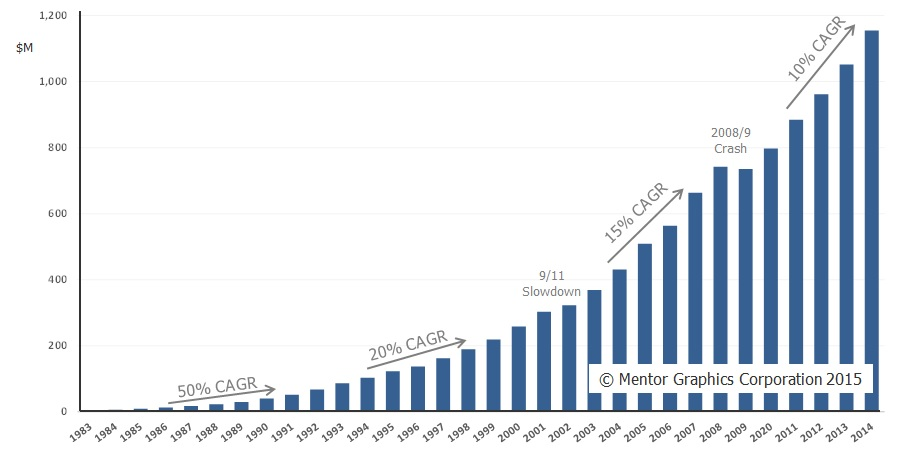
\includegraphics[width=1\textwidth]{figures/CFD_market.jpg}
    \caption{The global market size of CFD industry. From the early 1983, the market size has been increasing significantly reaching over 1200 million dollars by 2014. The trend has been predicted to continue. (Image from \cite{market_cfd})}
    \label{fig:cfd_market}
\end{figure}

As the definition says, CFD highly rely on computers, especially high-performance computers (HPC). Indeed, quite an objective part of HPC resource also goes to fluid dynamics simulation; see \ref{fig:break_down}. However, the simulation is becoming more demanding, and the CFD poses new challenges to HPC every year. For example, Formula 1 racing teams give high priority to aerodynamics simulation and they always want to run as much simulation as possible within a short period of time. If they want to beat the other F-1 teams in the aerodynamics, they need to run simulation faster in a more powerful supercomputer while the Fédération Internationale de l'Automobile (FIA) start to limit the power consumption of the CFD simulation \cite{formula1} of F-1 teams. Engineers like them from all areas face the similar challenge and they need to figure out a feasible way.

\begin{figure}[!tb]
    \centering
    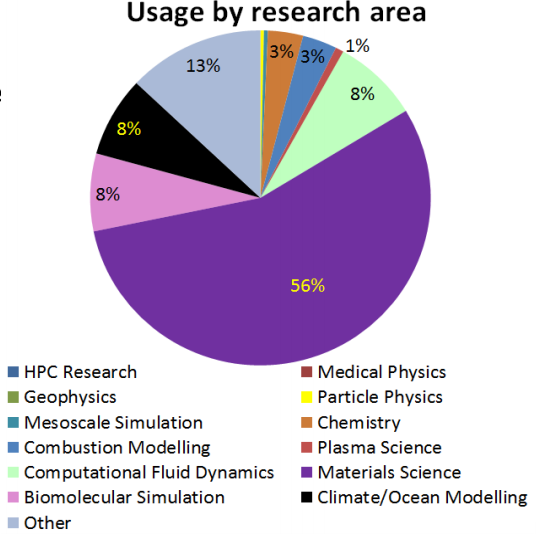
\includegraphics[width=0.7\textwidth]{figures/break_down.png}
    \caption{The HPC usage in ARCHER by research area in July 2016. Computational fluid dynamics related areas (including mesoscale simulation, combustion modeling and CFD) took over 10\% of the total use. (Image from \cite{archer_use}))}
    \label{fig:break_down}
\end{figure}


% \begin{figure}[!tb]
%   \centering
%       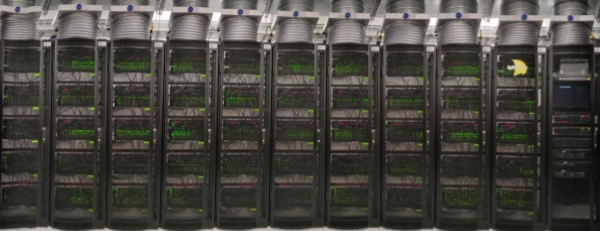
\includegraphics[width=0.7\textwidth]{figures/cluster.png}
%       \caption{The 500,000-core SpiNNaker \textit{102} machine at the University of Manchester (image from \cite{spinn-core}).}
%       \label{fig:cluster}
% \end{figure}


% Nowadays, the amount of data has grown increasing large, traditional computer architectures do not scale as the Moore's law. While parallelism is regarded as an option to keep the scaling, the SpiNNaker hardware was designed to be massively distributed and parallel. Thus the SpiNNaker hardware has the potential to be used as a parallel computing solution. As opposite to the traditional hardware, SpiNNaker has the following hardware features:

% \begin{itemize}
% \item \textbf{Manycore architecture}: though modern CPUs start to have multiple cores to gain some parallelism, the number of cores in a CPU is usually less than 10. On the opposite, a type Spinn-5 SpiNNaker board has 48 chips, which contains hundreds of ARM cores \cite{5th-summit}. Though there are more cores, because of the medium-performance (only 200MHz) ARM968 cores, the energy consumption stays relatively low.

% \item \textbf{Communication model}: the SpiNNaker cores communicate by sending message via UDP/IP \cite{ws6} and UDP/IP do not guarantee the delivery. Though it is the developers' responsibility to make sure the correctness, the developers do not need to worry about the dead-lock. It is designed as so because in a real human brain a neuron does not get any an acknowledgement when the communication is done \cite{spinnaker}.

% \item \textbf{Communication throughput}: extra performance might be gain from the reduce of the message size and more message can be process in the same amount of time\cite{furber2012overview}. Their link can transfer up to 31.25M byte/s, which means the links can handle 3M packets per second \cite{ws6}.\\
% \end{itemize}

Meanwhile, some neuromorphic hardware has been actively developed during the same period of time. SpiNNaker (Spiking Neural Network Architecture) is one of them. SpiNNaker  \cite{thespinnbible} is an approach to build a machine that is based to some degree on what is understood about the principles of operation of the human brain. It has the following hardware features:
\begin{itemize} 
\item \textbf{Massively parallel:} A single type Spinn-5 SpiNNaker board has 48 SpiNNaker chips. Each SpiNNaker chip has 18 ARM cores, which means the board has up to $48 \times 18 = 864$ cores. Each core has the ability to simulate at least 256 neurons. The SpiNNaker clusters are build with cabinets of boards. The SpiNNaker can bring massive parallelism.

\item \textbf{Low energy-consumption:} Opposite to the conventional HPC which are usually build up with energy-hungry cores running in GHz, the SpiNNaker only need 1 watt per chip.

\item \textbf{Communication model:} The communication model we primarily used is multicast. The cores can pass messages to multiple destinations by a single send.
\end{itemize}


In a word, the SpiNNaker has the full features as a supercomputer and it could provide new opportunities for parallel software engineers and CFD engineers. However, there is not much scientific applications developed on SpiNNaker, especially CFD applications. In this project, we will explore the potential of using SpiNNaker for CFD simulation and trying to achieve a good performance in terms of speed.\\
 
% On the other side, Computational fluid dynamics (CFD) is a science that, with the help of digital computers, produces quantitative predictions of fluid-flow phenomena based on the conservation laws (conservation of mass, momentum, and energy) governing fluid motion \cite{thelbmbible}. It help us to to solve real-world engineering problems, including aerospace engineering, meteorology, etc. However, CFD algorithm usually involve heavy computation. To get the simulation result in affordable time, scientists and engineers need to accelerate the simulation. Therefore, parallel computers including some supercomputers are heavily used for CFD simulation.\\

Lattice Boltzmann method (referred to as LBM in the rest of this report) is a mesoscopic CFD model which is recognized\cite{lbmmbook} as: (1) easy to apply to complex domain (2) No need to solve the Laplace equation (3) More importantly for this project, being naturally adapted to parallel processing due to the locality and explicit nature of the method. Due to its (3) nature, many parallel techniques are applied to accelerate the LBM simulation, including MPI\cite{he1999three}, OpenMP\cite{massaioli2002achieving} and GPGPU\cite{rogers1990upwind}, etc. \\

As we discussed above, the SpiNNaker has the ability to compute in massively parallel. Thus, there is a perfect match between the SpiNNaker and the lattice Boltzmann method. It is promising that we can get high performance and scalability in term of speed with SpiNNaker's low energy-consumption cores on the LBM simulation tasks, which is also the motivation behind this project.  \\




\subsection{Objectives} \label{sec:Obj}

Firstly, we can define our objective of this projects as follow:\\

\begin{quote}
Implementing a basic lattice Boltzmann method simulation on the SpiNNaker platform; and investigate its  performance and scalability in terms of speed. \\
\end{quote}

% KS: In point one there are two separate points which should be discussed seaparately. First, there is the implementation of the algirthm. Second, there
% is the use of a standard test problem to check that the implementation is
% working correctly. A wide range of test problems could be used.

% KS: There needs to be more here. It's not just a question of implementation. There
% needs to be some critical evaluation of ease-of-use, performance, and so on. 
% to add to KS. you need to discuss how your going to compare. speed, scale? energy? accuracy?

Firstly, we need to implement a standard lattice Boltzmann method on CPU as a reference, which can be more easily to understand and porting the algorithm; and we can also further evaluate the correctness, accuracy and compare the performance with this CPU implementation.\\

Secondly, we need to choose a pre-defined problem as the test problem from a wide range of the problems. As the test problem, it need to be generic and easy to check the correctness. To choose it, we take LBM model and the boundary condition into consideration, and, finally, a two dimensions and nine vectors (D2Q9) model with a periodic condition problem described by Minion and Brown \cite{minion1997performance} was chosen. It is generic -- D2Q9 model is widely used, and easy to check the correctness -- with the mentioned initial condition, there will be a turbulence in a fix step and we can check it.\\

Then, we focus on the design and implementation of the LBM on the SpiNNaker. For each step of the LBM, we need to carefully design and implement, especially for the communication in SpiNNaker with the SpiNNaker software stack \cite{software_spinn}. This is also the main part of this project.\\

Finally, after implementing the simulation on SpiNNaker, we will to evaluate correctness and accuracy the simulation result by compare the numbers in quantitatively. After we confirm the correctness, them some experiment would be focus on optimization the communication and bench mark the result with the standard CPU implementation on speed-ups and scalability.\\

\subsection{Project Overview}

The work of this project are threefold:\\

 \textbf{A basic lattice Boltzmann implementation on CPU}: we firstly built a standard serial implementation of a pre-defined lattice Boltzmann scenario described by Minion and Brown \cite{minion1997performance}; see Subsection \ref{sec:ip}. \\

 \textbf{A basic lattice Boltzmann implementation on SpiNNaker:} after we implemented the simulation on CPU, we used the CPU implementation as a reference to implement the same simulation on SpiNNaker platform with some of the SpiNNaker software development kit; see Section \ref{sec:dai}\\

\textbf{An investigation on the speed performance and scalability}: we demonstrate that lattice Boltzmann on SpiNNaker platform offers better speed performance in larger scale when compared to CPU and it also has a good scalability on weak-scaling. We bench-marked two implementations of the lattice Boltzmann method scenario: the first one is the standard implementation of on a normal Intel CPU and second one is a implementation on SpiNNaker mentioned above. The observation shows that lattice Boltzmann program can gain  $277.192 / 60.01 = 4.61$ speed-up in terms of speed over a certain scale; see Section \ref{sec:perfe}.




\newpage
\section{Background} \label{sec:bg}


This section will provide a basic background information of history neuromorphic computing (\ref{sec:sb}) and the SpiNNaker (\ref{sec:sa}) in hardware architecture (\ref{sec:sa}) and software stack (\ref{sec:sss}). Then this section will explain some important conceptions in physics (\ref{sec:PB}) about the lattice Boltzmann method: why it is necessary and how it works. 


\subsection{History} \label{sec:sb}
The vision of \textbf{neuromorphic computing}\cite{mead1980introduction} is to enable a new generation of computer architecture, designing energy-efficient general-purpose computing systems comparable to the human brain. In 1989, Carver Mead from Caltech first introduced the concept of \textit{neuromorphic Engineering} \cite{mead1980introduction}. From 1990 to 2003, the Von Neumann-based CPU industry continued to grow, Moore's Law \cite{schaller1997moore} was reaching its limits, and neuromorphic computing was dormant for more than a decade. In around 2004, the frequency growth of single-core processors slowed down, and IC designers turned to multi-core processors. Academia began to look for alternative technologies to the Von Neumann architecture.\\

In 2004, Kwabena Boahen from Stanford University developed Neurogrid \cite{benjamin2014neurogrid}, an analog circuit-based neural chip. In 2005, the University of Manchester began to develop \textbf{SpiNNaker}, a multicore neural supercomputer based on ARM chips. In the same year, the Europe, the US and IBM started their neuromorphic computing projects: FACETS project \cite{meier2004fast}, SyNAPSE project\cite{park2014impact} and Blue Brain project\cite{gara2005overview}, respectively. \\

In 2013, A 10-year-project, \textbf{Human Brain Project} began in 2013. It aims at building a research infrastructure to help advanced neuroscience, medicine, and computing \cite{hbp}. Although, the SpiNNaker project had started even before the Human Brain Project funded by the \textit{Engineering and Physical Sciences Research Council} (EPSRC), the Human Brain Project bring more funding and brilliant researchers building the 1 mio core SpiNNaker machine since November 2018; see Fig~.\ref{fig:super_machine}.

\begin{figure}[!tb]
   \centering
       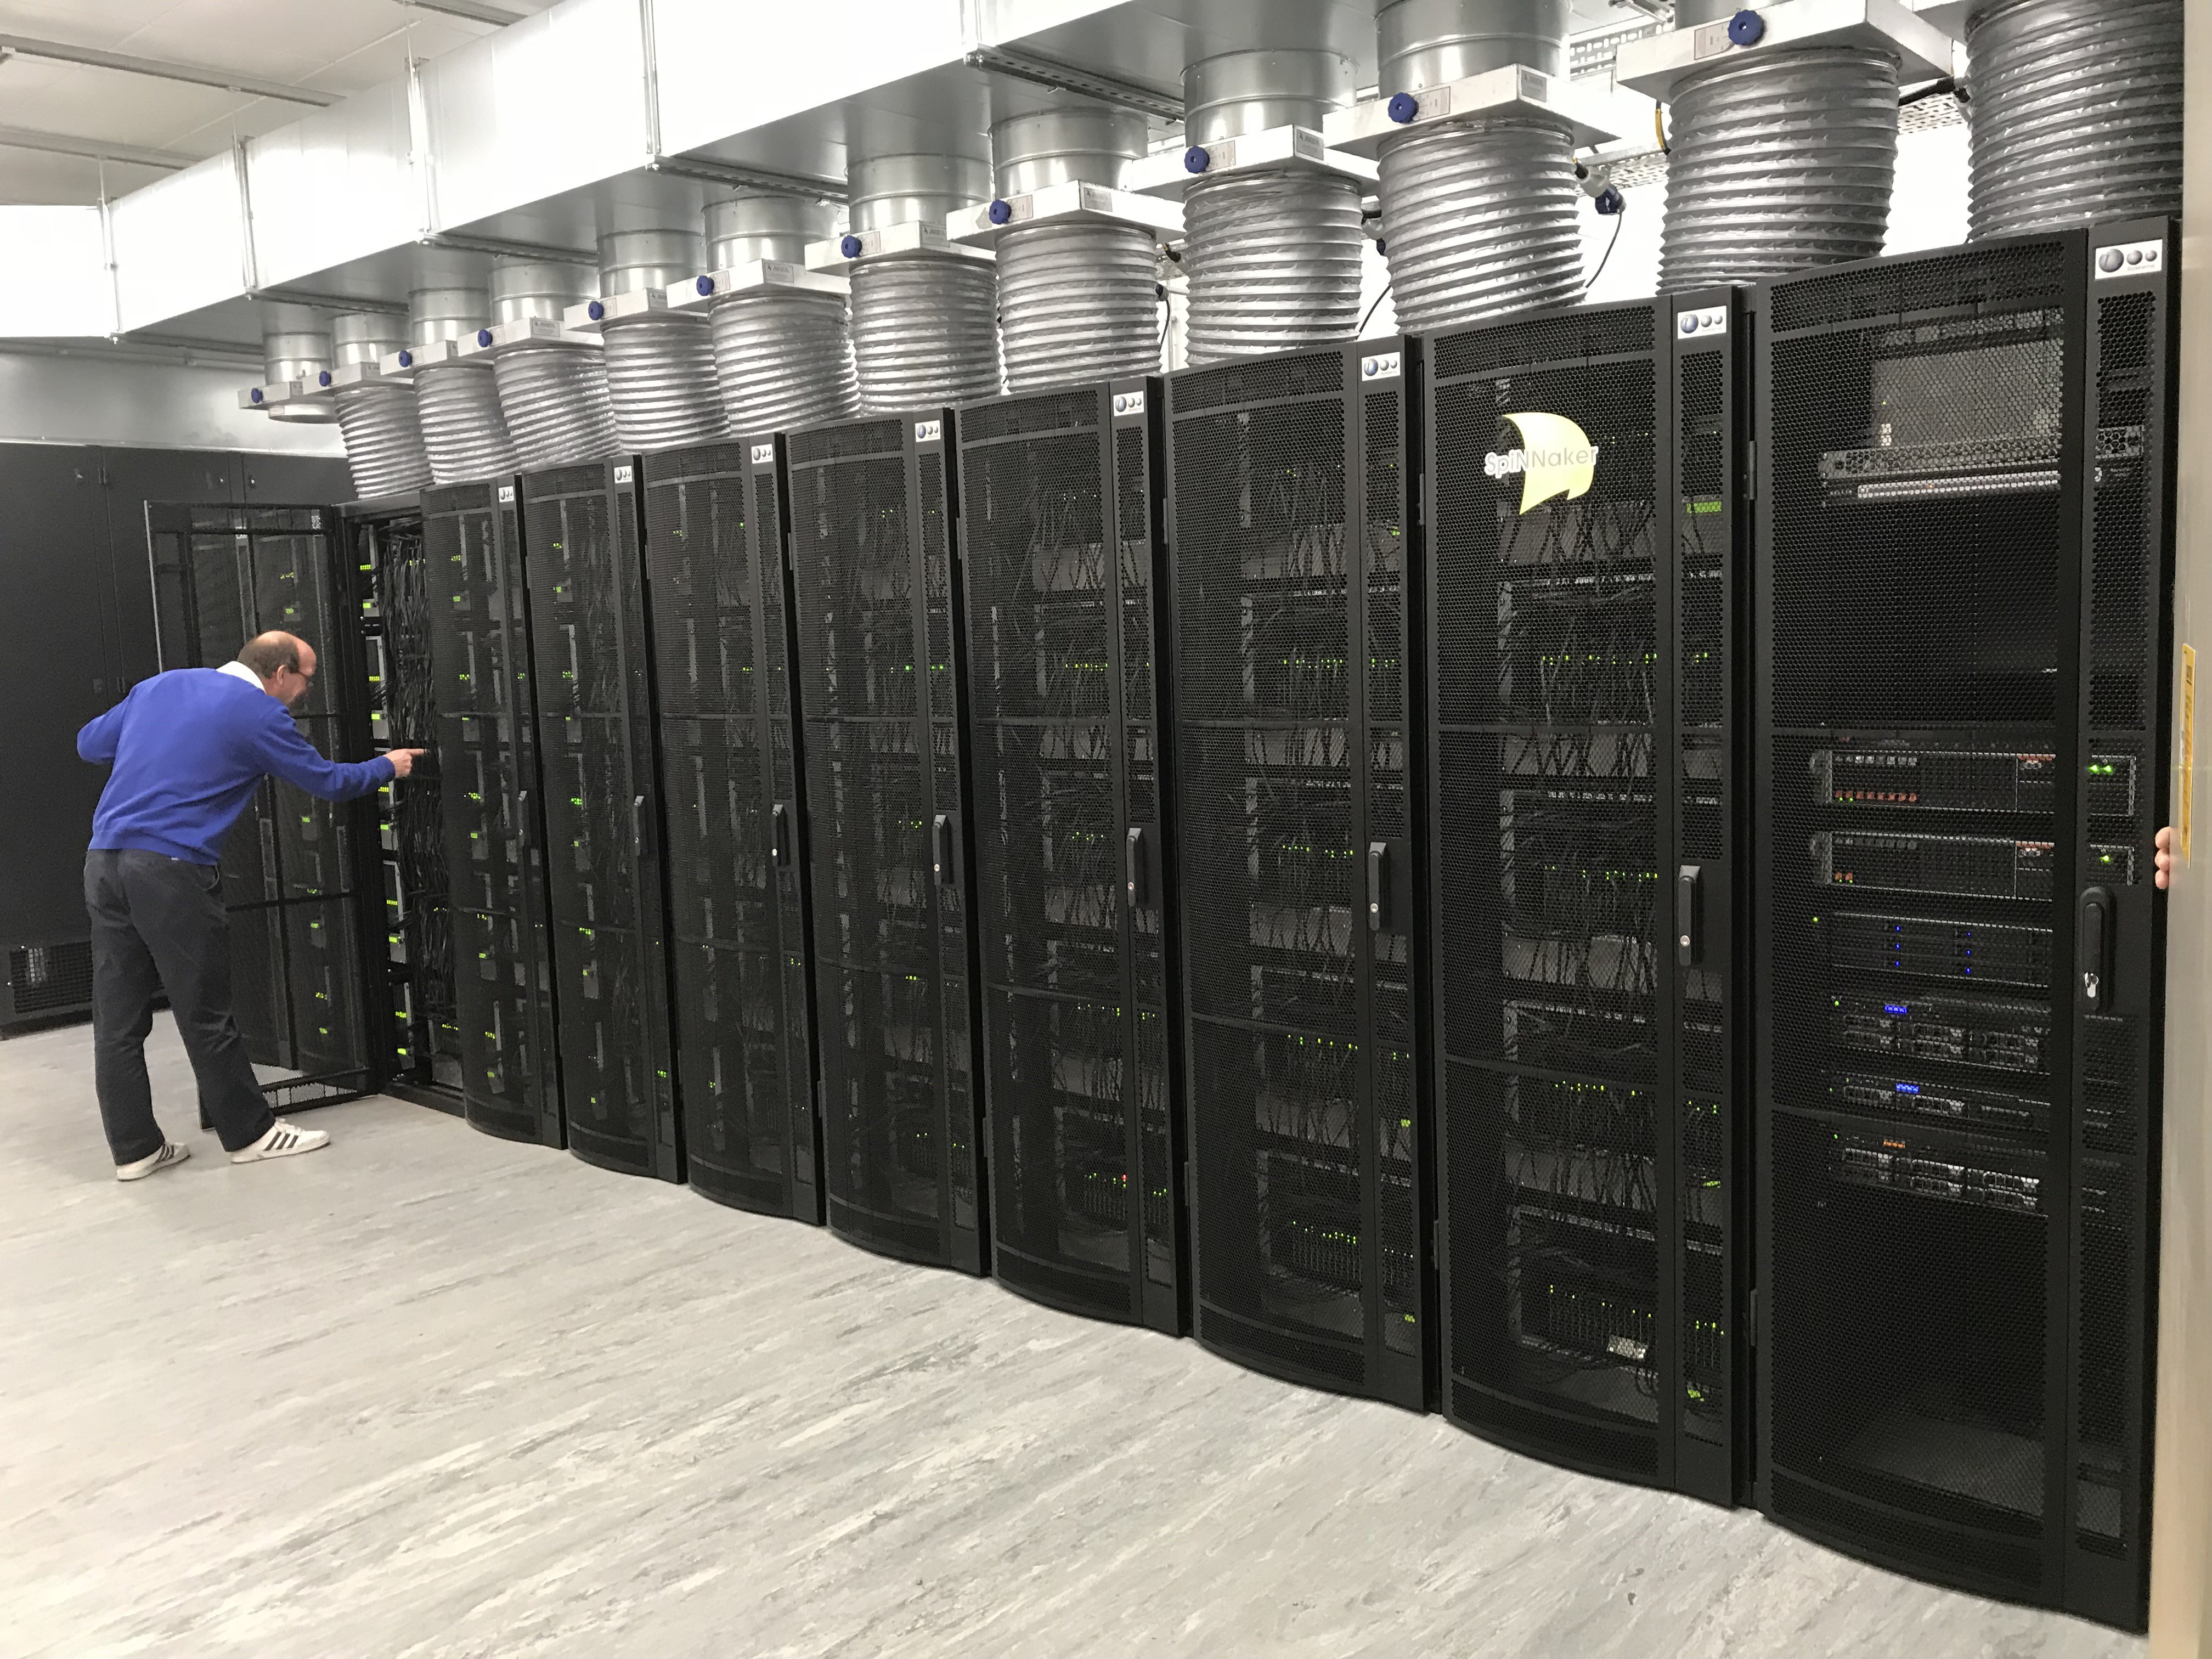
\includegraphics[width=0.8\textwidth]{figures/super_machine.jpg}
       \caption{Since November 2018: The 1 mio core SpiNNaker HBP Platform machine((image from \cite{super_machine})).}
       \label{fig:super_machine}
\end{figure}



\subsection{SpiNNaker Architecture} \label{sec:sa}
\subsubsection{Chip Architecture}
\begin{figure}[!tb]
   \centering
       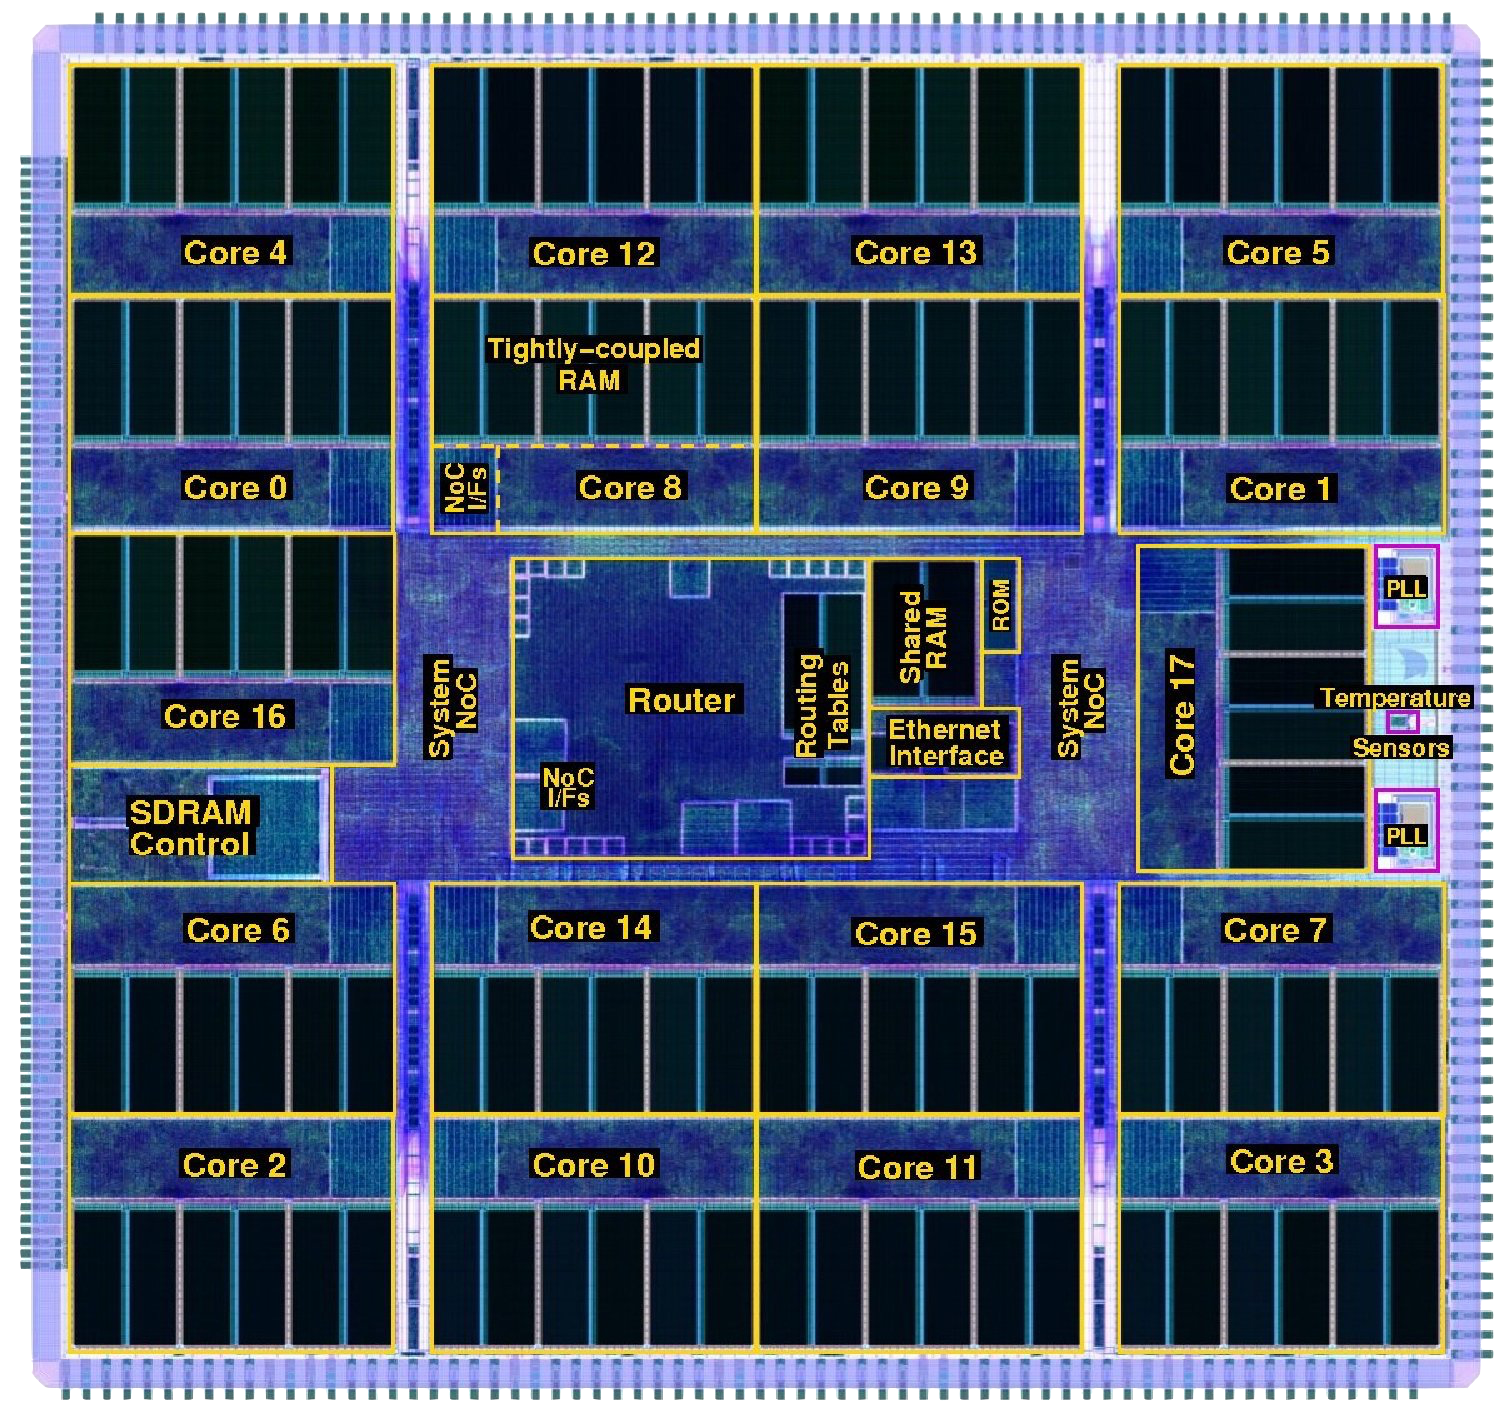
\includegraphics[width=0.8\textwidth]{figures/spinn_labeled_bw.png}
       \caption{An 18 cores SpiNNaker chip ((image from \cite{spinn-core})).}
       \label{fig:spinn-core}
\end{figure}
Fig.~\ref{fig:spinn-core} shows the die plot of an 18 ARM cores SpiNNaker chip. It mainly consists of \cite{furber2012overview}:

\begin{itemize}
    \item \textbf{ARM968 core:} there are 18 ARM968 cores in the chip. Being different from the most cores in the PCs or supercomputer running at $\sim GHz$, ARM968 is a medium-performance computing unit running at 200MHz with 220 DMIPS \cite{furber2012overview}. There are two very limited tightly coupled memory (TCM) blocks: a 64 Kbytes of data tight-coupled memory (DTCM) block and a 32 Kbytes of instruction tight-coupled memory (ITCM) block; see Fig.~\ref{fig:arm_968}. Other controllers including direct memory access (DMA) controller, communication controller, vectored interrupt controller are also built in. A major difference from the most cores in the market is that the ARM968 core do not have floating-point hardware and use fixed-point arithmetic instead. Though I might be more energy-efficient, it bring greater challenge to programmers \cite{furber2012overview}. Luckily, a software floating-point arithmetic is supported, though the performance might be slower and more memory-hungry \cite{spin-chip-resources}.
    \begin{figure}[!tb]
   \centering
       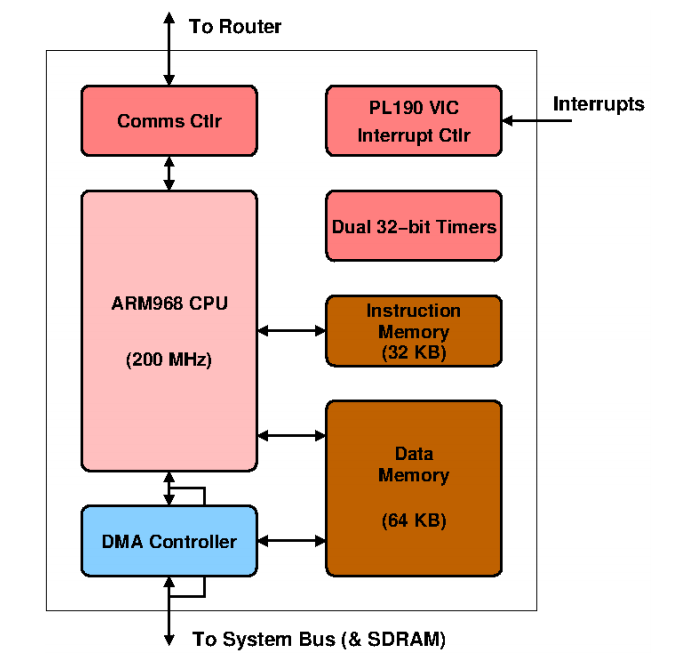
\includegraphics[width=1\textwidth]{figures/core.png}
       \caption{A diagram of SpiNNaker Core -- ARM 968 ((image from \cite{spin-chip-resources})).}
       \label{fig:arm_968}
    \end{figure}
    
    \item \textbf{Ethernet:} the SpiNNaker system connect to a host machine via Ethernet links \cite{furber2012overview}. Though an Ethernet MII (Media Independent Interface) is built-in each of the cores, only one core per board is using this interface. In term of speed, the Ethernet support around 10 Mbyte/s \cite{spin-chip-resources}. In type Spinn-5 board, there are extra three FPGAs (Field Programmable Gate Arrays) connected via SATA link which enable a higher bandwidth in this case. 
    
    \item \textbf{Router\label{sec:router}:} SpiNNaker cores communicate via passing message, where we call it "packet". When the SpiNNaker is running, there is a large number of packets going in and out each core, and, unlike the other message-passing framework in HPC, SpiNNaker cores send packets via a packet-switch network optimised for large numbers of small fixed-sized packets sent over the UDP/IP protocol. The Routers are responsible for put packets in and out. More communication details would be covered in Section \ref{sec:dt}.
    
    \item \textbf{System RAM:} When booting the machine, one of the core is elected to be a special processor as \textbf{Monitor Processor}. The rest cores are available for the application processing. For each chip, there is a 32Kbytes of System RAM used by either by the Monitor Processor when running neural network simulation or by all the cores when running non-neural simulation.
    
    \item \textbf{Sensors:} each SpiNNaker chip contains three temperature sensors, which are used to limit the clock rate when the temperature of chip rises too high.
\end{itemize}
\subsubsection{Network Topology}
Before we talk about how the SpiNNaker cores communicate, we need to illustrate how they are connected with its network topology.

In a SpiNNaker board, SpiNNaker chips are organized as a 2-dimension mesh network with bidirectional links to their six neighbours \cite{testchip} TODO: A DESCRIPTION ON THE NETWORK TOPOLOGY, A DIAGRAM NEEDED

\subsubsection{Data Transmission in SpiNNaker} \label{sec:dt}
As we introduced before, SpiNNaker cores communicate with each other by passing message (packets). Each packet is of 40bits or 72bits (with a 32bits payload) \cite{furber2012overview} and there are four kinds\cite{ws6} of packet:

\begin{itemize}
    \item \textbf{Multicast (MC) packet:} Multicast is the primary communication format used by the SpiNNaker application developers. With this method, the packets are sent once to multiple destinations; see Fig.~\ref{fig:multicast}  The routing key is allocated by the SpiNNaker system runtime. 
    
    As Fig.~\ref{fig:mc_pkt_layout} shows, a multicast packet contains an 8bits control header, a 32bits routing key and an optional 32bits payload. TODO: A disruption of MC packets
    
    \begin{figure}[tb]
    \centering
    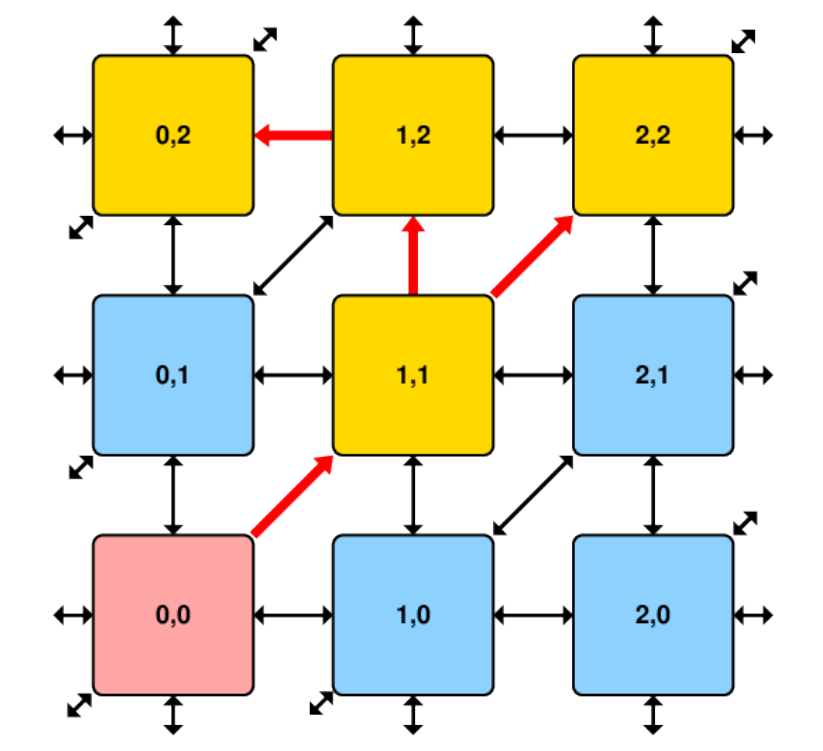
\includegraphics[width = 0.8\hsize]{figures/multicast.png}
    \caption{A Multicast show case, where core (0,0) send packet once to multiple destinations, core(1,1), core(1,2), core(0,1) and core(2,2).(image from \cite{ws6}).}
    \label{fig:multicast}
    \end{figure}
    
    \begin{figure}[tb]
    \centering
    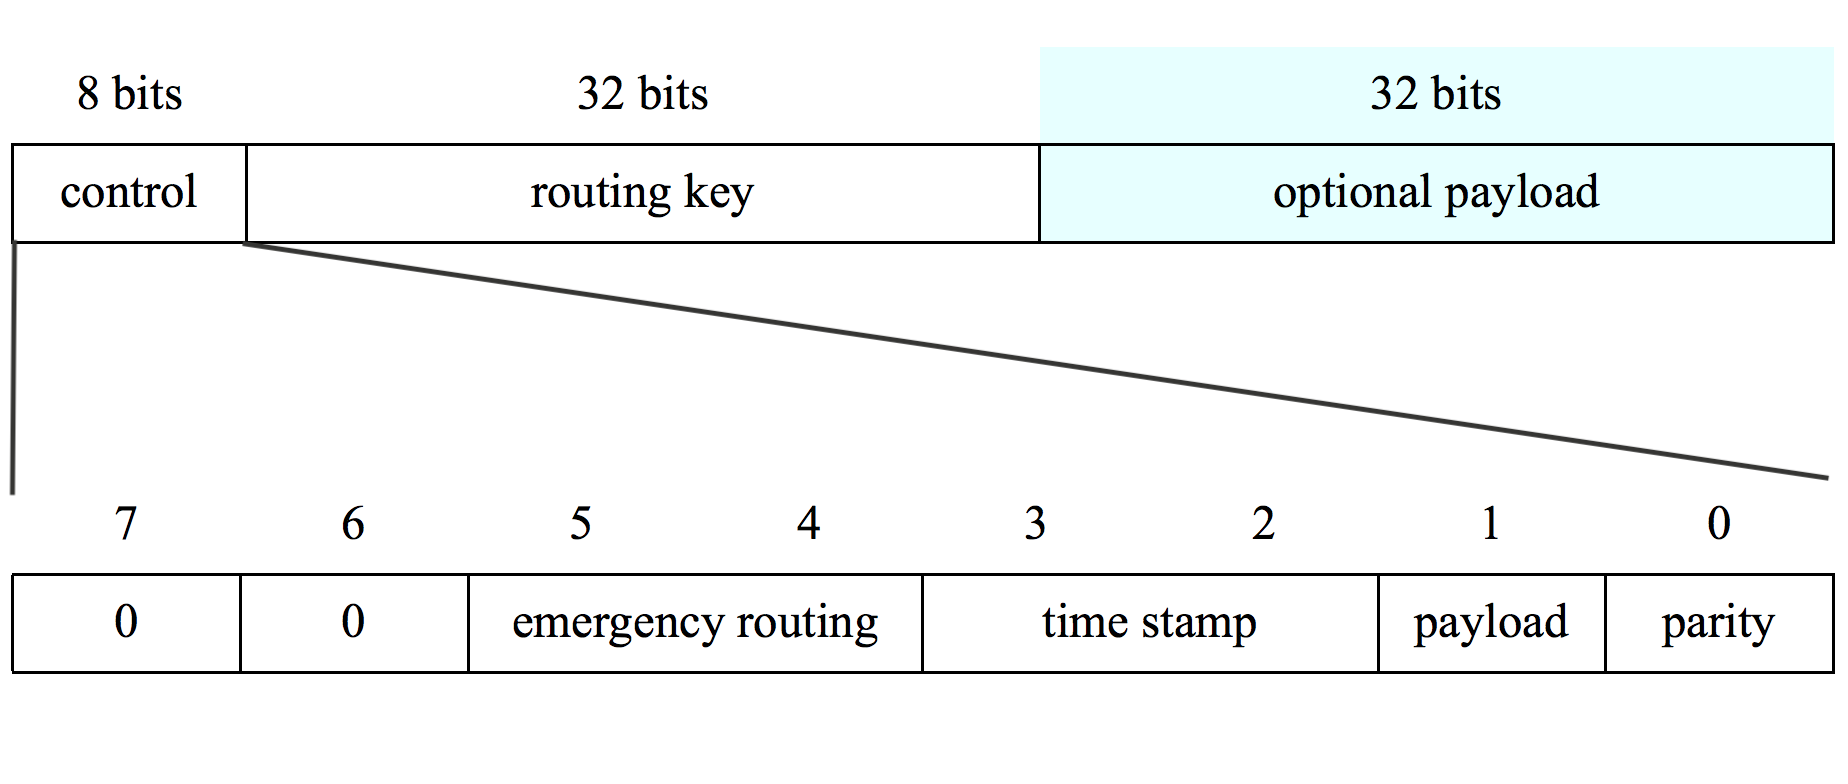
\includegraphics[width = 1\hsize]{figures/mc_pkt_layout.png}
    \caption{SpiNNaker Multicast Packet Space (image adapted from \cite{mc_pkt_layout}).}
    \label{fig:mc_pkt_layout}
    \end{figure}
    
    \item \textbf{Point-to-point (P2P) packet:} Point-to-point method is sending packets from a source core to a destination core. This method mainly used as system management.
    
    \item \textbf{Nearest-neighbour (NN) packet:} Nearest-neighbour method in SpiNNaker is unicasting or broadcasting data to neighbours i.e. six directly connected chips.
    
    \item \textbf{Fixed-route (FR) packet:} fixed-route method is sending packets from the SpiNNaker device to the host system. This method is mainly used as sending debugging data from a core back to the host machine.
\end{itemize}

As we discuss before, the SpiNNaker cores communicate over UDP/IP protocol. Thus \textbf{none of those four communication method guarantee the deliver of packets}, and as a consequence, the packets might be drop at any time. This situation may be exacerbated when there is a big amount of packets in the communication fabric. It is reasonable as in human brain, the spikes might be lost. However this characteristic brings difficulty for developing high-performance computing application, especially for those which are involved in huge message-passing. We will discuss the difficulty and solution at Section~\ref{sec:ssc}.

\subsection{SpiNNaker Application Development} \label{sec:sss}
\subsubsection{SpiNNaker Software Stack}
    \begin{figure}[!tb]
        \centering
       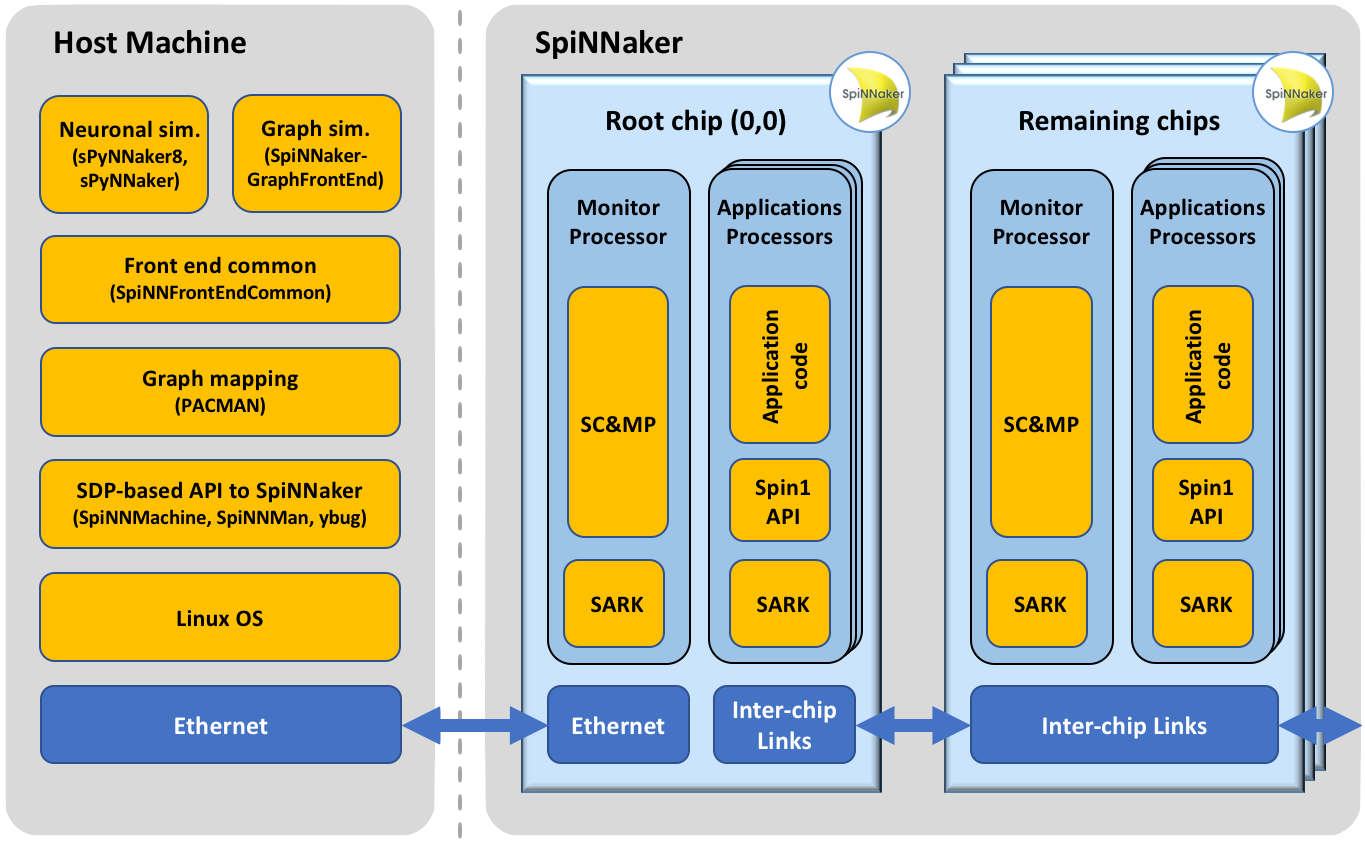
\includegraphics[width=1\textwidth]{figures/software_stack.png}
       \caption{A diagram of SpiNNaker Software Stack ((image from \cite{spin-chip-resources})).}
       \label{fig:software_stack}
    \end{figure}

Fig.~\ref{fig:software_stack} shows what SpiNNaker software contains and how it works. High-level abstractions for Neural simulation (\textit{sPyNNaker}) and general parallel computing (\textit{SpiNNaker GraphFrontEnd}) provide APIs for developers to describe the neural connection or computational graph. Since we are not developing neural simulation application, the primary software we used for this project is the SpiNNaker GraphFrontEnd. 

After the computational graph is described by the developers in Python, the Partition and Configuration Manager system (\textit{PACMAN}) will map the computational graph to the SpiNNaker cores. 

The actual computation of each vertex is defined via the \textit{Spin1} API in C code. Both of the partition information and the pre-compiled computation job are transferred to the root chip of SpiNNaker machine via Ethernet. Then the information would be passed to the rest of the chip in the board via  the inter-chip connection.


Sitting on the lowest layer of the software stack, the SpiNNaker application runtime kernel (\textit{SARK}) support the runtime system of the SpiNNaker core. 


\subsubsection{SpiNNaker Development Workflow} \label{sec:sdw}

For this project, instead of neural simulation, we are using the SpiNNaker as a parallel computer and our workflow of development are using the GraphFrontEnd API.

Firstly, even before we define the computation of each individual vertex, we need to define the data specification information such as what data we are going to pass to the SpiNNaker, how many router keys does a vertex may want via the \textit{SpiNNFrontEndCommon} and \textit{PACMAN} API. After we define our vertex, we need to define the edge between the vertex via \textit{PACMAN} API.

Then we need to express our communication fabric as a graph by connecting the vertices together with the edge we just defined via the \textit{SpiNNaker GraphFrontEnd} API in Python. 

After we got our computational graph, we then need to define the computation and communication of each individual vertex in C via the \textit{Spin1} and \textit{simulation} APIs, etc.

\subsection{Development Environment for SpiNNaker} \label{sec:impl}
At the beginning of this project, our first choice to access the SpiNNaker machine is to use a directed connected broad for development. However, later on, there is problem with the connection port. Due to the pandemic COVID-19, the repair is not available. We then switch to the web interface with the Jupyter Notebook. There are many ways to get access to the SpiNNaker machine, we will mainly discuss those two method that are used during this project.
\subsubsection{Directed Connected Board with IDE}
The first choice for this project is to run the simulation with physically board connecting with the laptop. As shown in the Fig.~\ref{fig:laptop}, SpiNNaker developers can make all the development offline. Typically, they write code in their host computer with a code editor or an IDE then offload the simulation to the connected SpiNNaker board.\\

One of the advantages of development with a SpiNNaker Board is that the developers can physically watch the running condition of the SpiNNaker boards and make corresponding manipulation. Another advantage is that the developers can make full use of their favourite code editors or IDEs (see Fig.~\ref{fig:ide}), which makes it easier to view the source code and debugging.\\

There are some disadvantages though. A major disadvantage is that it is the developers' duty to maintain the development condition of the SpiNNaker board including the Ethernet connection, electronic power and the condition of the SpiNNaker board itself. Most SpiNNaker users are not professional electronic engineers, so if there is any trouble with those problem, the developers must try to get help from the SpiNNaker team or they are on their own. \\

\begin{figure}
\centering
\begin{subfigure}[tb]{1\textwidth}
   \centering
       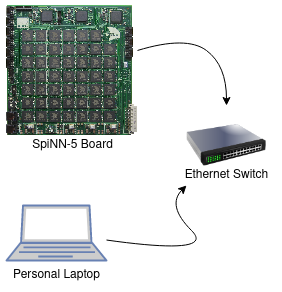
\includegraphics[width=0.8\textwidth]{figures/laptop.png}
       \caption{Development with Directed Connected Board ( board image from \cite{spinn-core}).}
       \label{fig:laptop}
\end{subfigure}

\begin{subfigure}[tb]{1\textwidth}
   \centering
       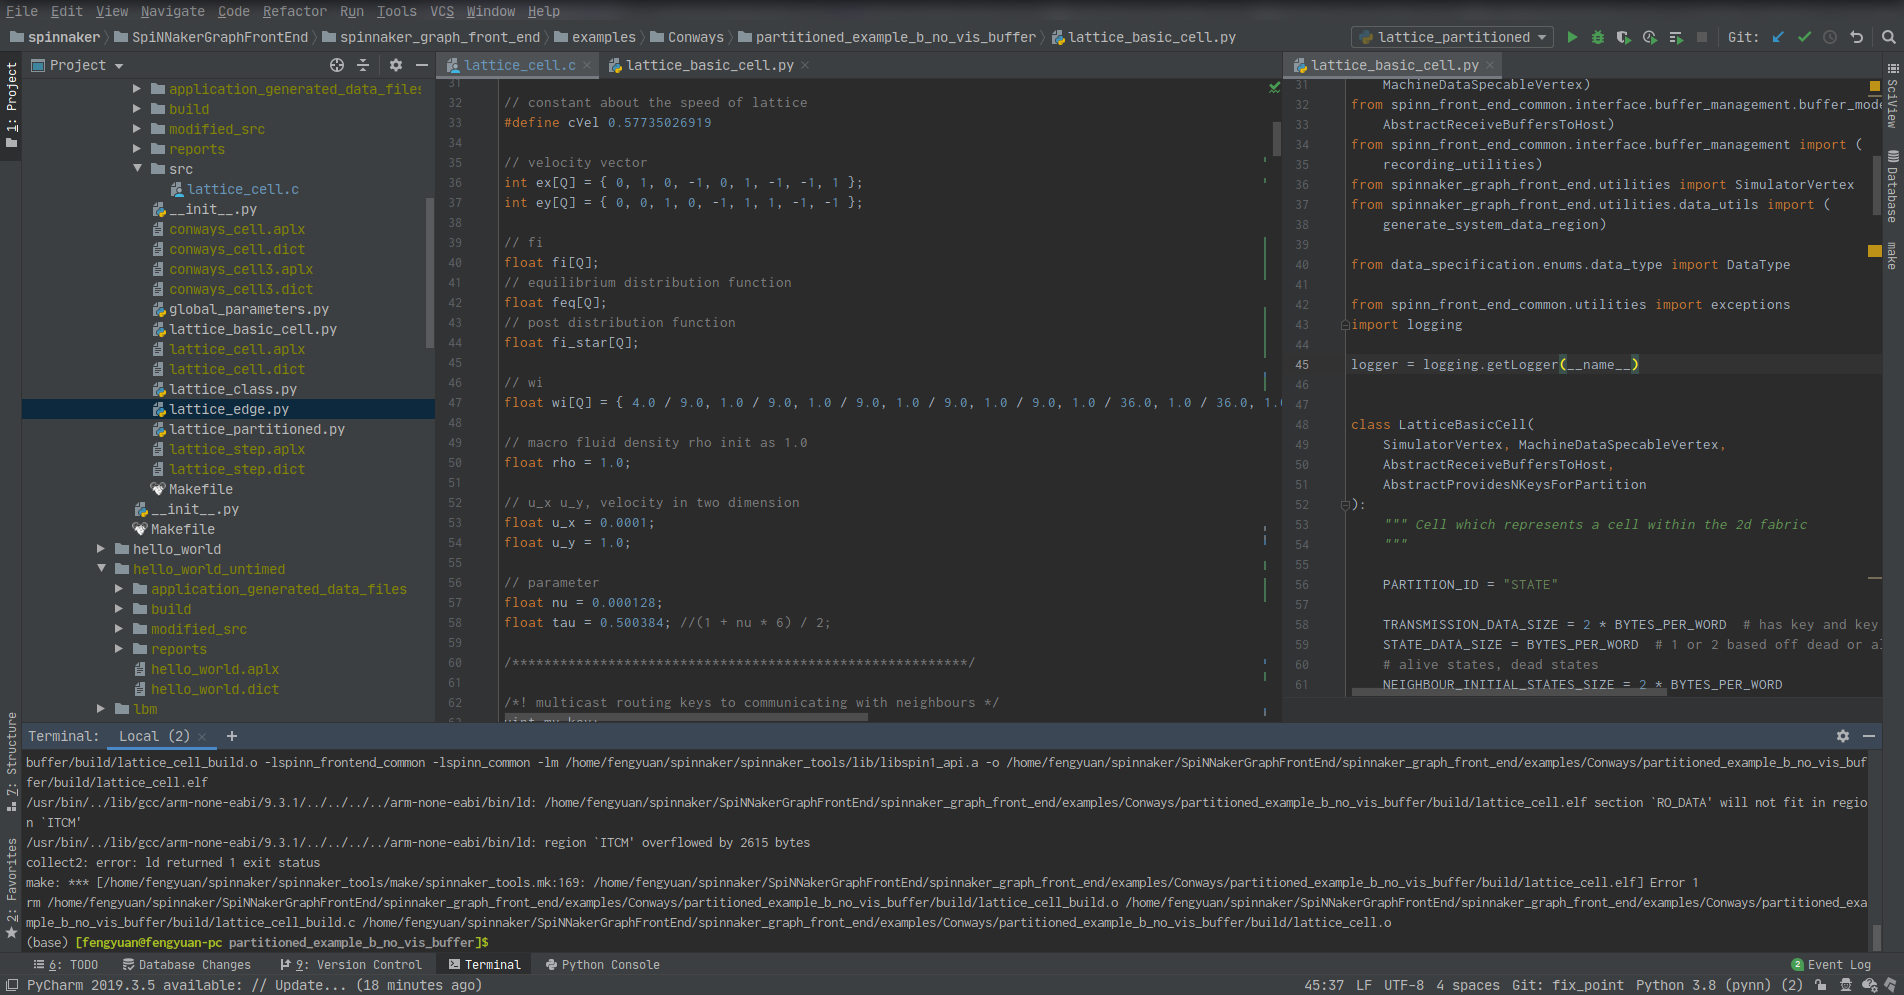
\includegraphics[width=1\textwidth]{figures/ide.png}
       \caption{Development with Directed Connected Board in an IDE.}
       \label{fig:ide}
\end{subfigure}

\caption[]{}
\end{figure}


\subsubsection{Web interface with Jupyter Notebook}
For most SpiNNaker users or who are just get into the SpiNNaker development, they may not even have a board. The best way to write SpiNNaker to develop SpiNNaker application is using the web interface development by the SpiNNaker team. \\

With the web interface, the developers run the python code within the Jupyter Notebook. The Jupyter also provides a terminal enabling the developers compile their C code and run shell command. For this project, we compile the C code on the laptop and upload the binaries to the remote system and run the application in the Jupyter notebook(shown in Fig.~\ref{fig:jupyter}).\\

The biggest advantage of developing with the Jupyter interface is that the developers do not need to take extra concern on the board maintain. They can pay full attention on the application development even if they do not even have a board. Another advantage is that there are more than 1 million cores available remotely. They developer can scale their application up with the Jupyter notebook easily. Though it might be easier for developer to connect with a SpiNNaker machine via the Jupyter, it is hard to view the source code of the APIs and debugging in the Jupyter. \\

Overall, for hardcore developers or absolute beginners, it might be better to use the connected board to develop SpiNNaker framework or applications and getting familiar with the SpiNNaker API stack. For those who have been already familiar with the SpiNNaker API stack and want to scale their application up, it might be better to use the Jupyter interface.\\

For this project, our first choice was using a directed connected Spinn-5 board and an IDE on the laptop. Later on, in the second half of this research, the connection between the board and the laptop started to become unstable. We then decided to switch to the Jupyter interface.\\

\begin{figure}[!htbp]
\centering
\begin{subfigure}[!htbp]{1\textwidth}
    \centering
   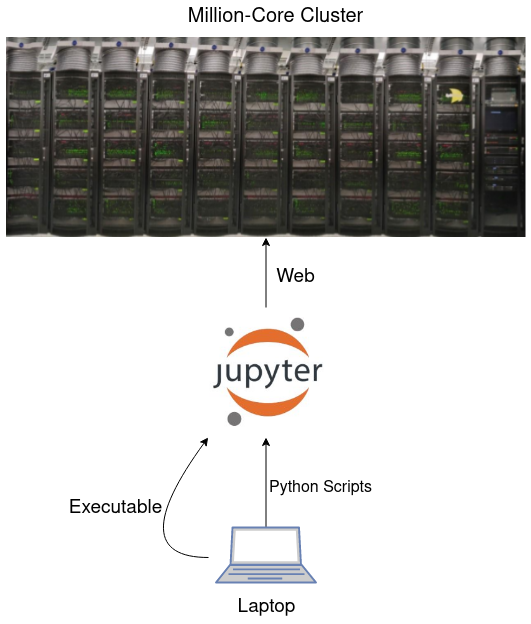
\includegraphics[width=0.8\textwidth]{figures/jupyter.png}
       \caption{Development with Jupyter Web interface ( board image from \cite{spinn-core}).}
       \label{fig:jupyter}
\end{subfigure}

\begin{subfigure}[!htbp]{1\textwidth}
    \centering
   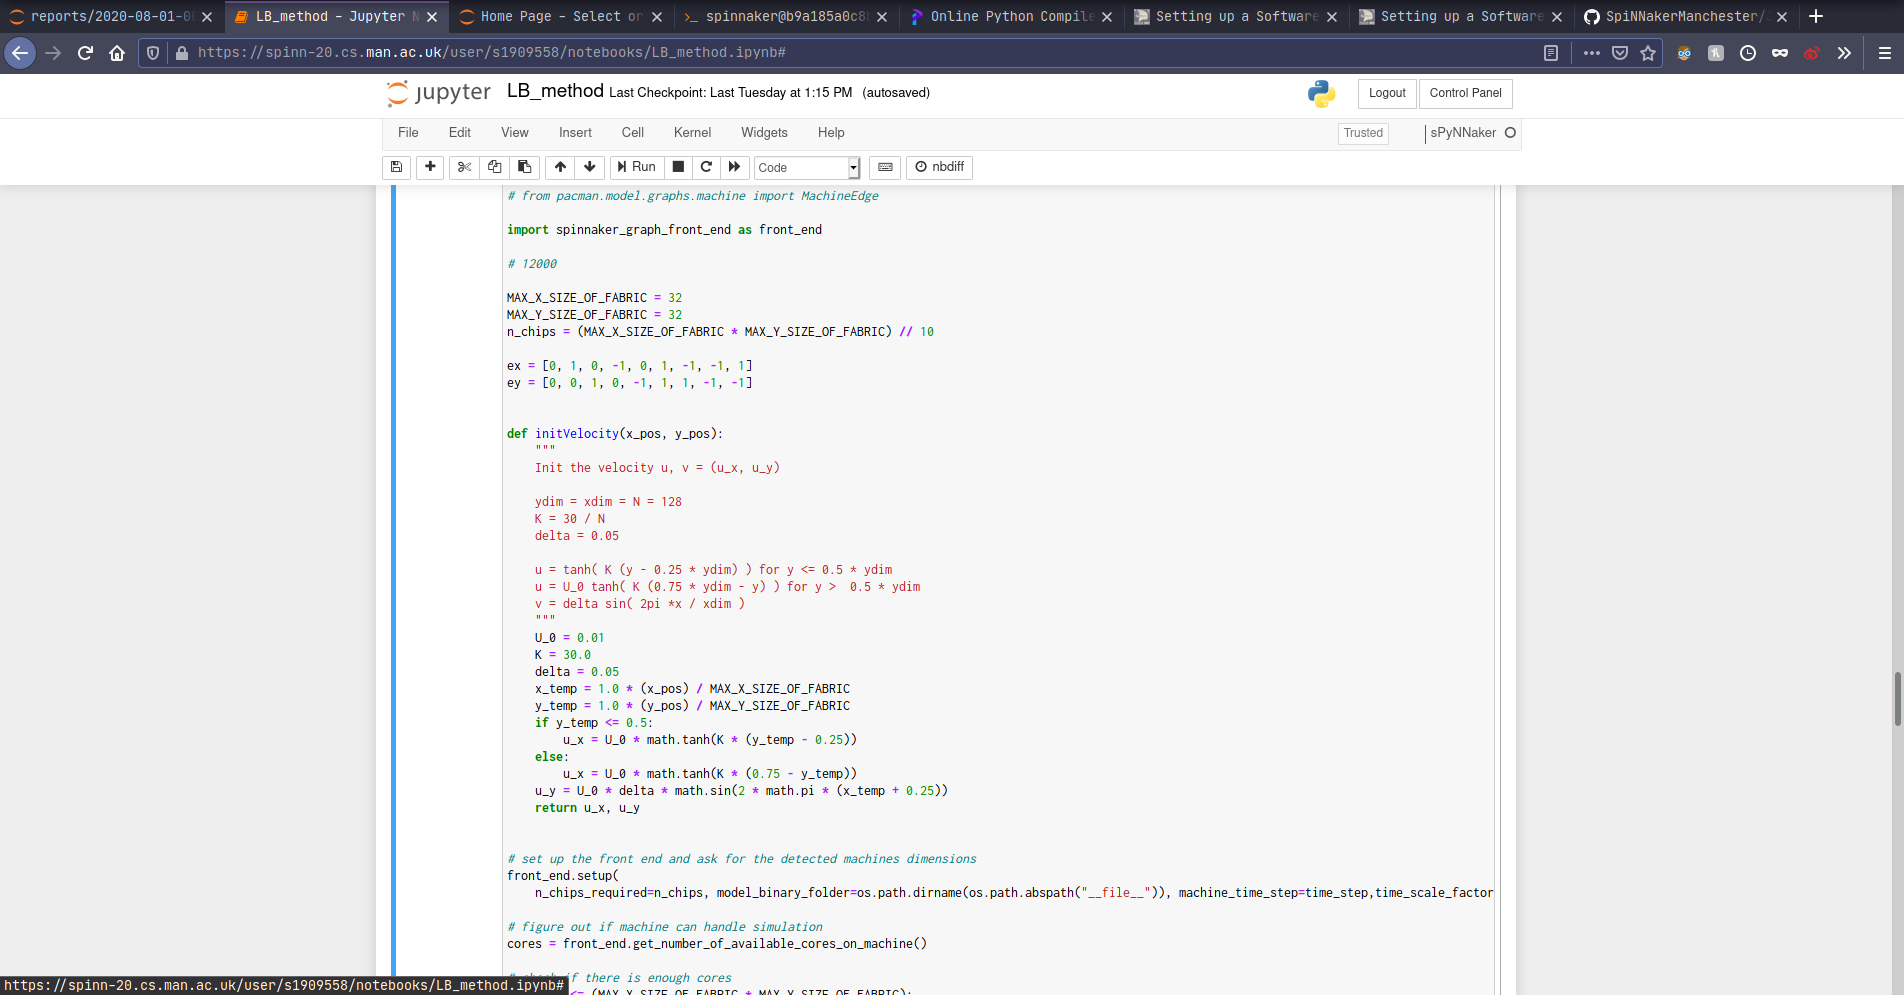
\includegraphics[width=1\textwidth]{figures/jupyter_dev.png}
       \caption{Development Environment in Jupyter}
       \label{fig:jupyter_dev}
\end{subfigure}

\caption[]{}
\end{figure}


\subsection{Physics Background} \label{sec:PB}
% KS: Need to clearly separate what is the kinetic theory of gases and the Boltzmann
% equation, and what is lattice Boltzmann. REFERENCES?

% KS: What are the Navier Stokes equations?
\subsubsection{Fluid Model in Brief}
Fluids are physically discrete systems composed of a large number ($~10^{23}$) of particles \cite{lbmmbook}, where every particle is constantly doing Brownian motion \cite{karatzas1998brownian} and exchange momentum and energy by collision. Thus the micro structure and motion are quite complex in both space and time. On the other hand, contrary to the inhomogeneity, dispersion, and randomness of microscopic motion, the macroscopic motion of the fluid exhibits uniformity, continuity, and determinism. The macroscopic motion and other properties of the fluid are the result of averaging the microscopic motions of the fluid molecules. Therefore, the mathematical models describing fluid motion can vary considerably when observed at different scales.\\

In general, methods for describing fluid systems can be classified into Molecular Dynamics model, Mesoscopic Model and macro continuum models depending on the scale \cite{karatzas1998brownian}; see Fig.~\ref{fig:fluid_models}. The Molecular Dynamics model views the fluid as a many-body system consisting of a large number of molecules and focuses on the dynamic behavior of each fluid molecule (at \ref{sec:HE}). Through the movement of each molecule of the statistical representation to describe the overall motion of the fluid; macroscopic continuum model of the fluid as a continuous whole, focusing on the fluid micro-group, with a set of partial differential equations (Navier Stokes Equations \ref{sec:nse}) to describe the macroscopic motion of the fluid; meso-dynamic model, including the lattice Boltzmann model, focuses on the velocity distribution function of the fluid molecules, by expressing its macroscopic physical quantities and distribution function over time to obtain macroscopic flow Information (Boltzmann Equation \ref{sec:BE}). \\

\begin{figure}[!tb]
   \centering
       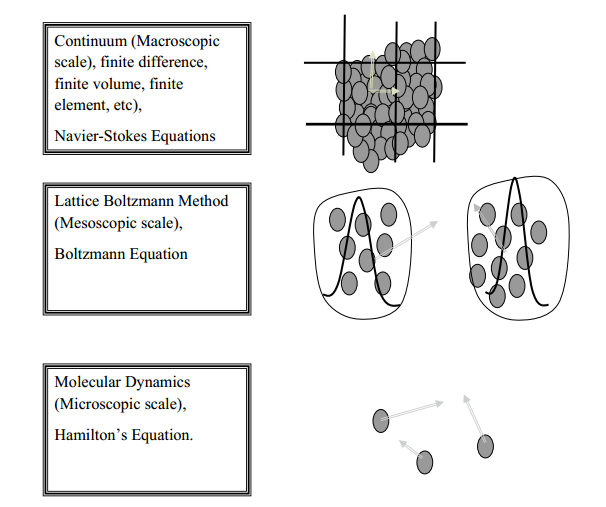
\includegraphics[width=1\textwidth]{figures/fluid_model.png}
       \caption{Three different kinds of fluid models (image from \cite{karatzas1998brownian}).}
       \label{fig:fluid_models}
\end{figure}

The lattice Boltzmann method (LBM) as a mesoscopic model set in the between the microscopic model and the continuum model. It enjoy the advantages of both the macroscopic and micropic approaches, and we will introduce both of them next before the LBM.

\subsubsection{Navier-Stokes Equations} \label{sec:nse}
In general, a fluid can be viewed as a continuous medium that fills the entire flow field, so that the physical quantities of density, velocity, temperature, etc. can be defined at each point of the flow field and a series of partial differential equations can be established to describe the motion of the fluid. The continuous medium assumption is a fundamental assumption of fluid mechanics and is an approximate treatment of macroscopic fluid structure.\\

Based on the assumption of a continuous medium, the motion of a fluid follows the law of conservation of mass, momentum and energy, which can be mathematically described by a set of partial differential equations Equation.~\ref{equ:NS}:

\begin{equation}
    \left\{\begin{matrix}
\frac{\partial \rho}{\partial t} + \triangledown \cdot (\rho u) = 0\\ 
\\
\frac{\partial (\rho u)}{\partial t} + \triangledown \cdot (\rho u u) = 0\\ 
\\
\frac{\partial (\rho u)}{\partial (t) + \triangledown \cdot (\rho u e)} = \sigma : \triangledown u - \triangledown \cdot q
\end{matrix}\right.
\label{equ:NS}
\end{equation}

Here in Equation ~\ref{equ:NS}, $\rho$, $u$, $T$ and $e$ are the density, speed, temperature and internal energy per unit mass, respectively. $\sigma$ is the strain tensor and $q$ is the heat flux from heat transfer and heat radiation.

The Equation ~\ref{equ:NS} is not in closed-form. In order to obtain the complete equations, the equations of states need to be supplemented with the relationship between the stress tensor and the rate of deformation tensor, between the heat flow vector and the temperature gradient, and with the thermodynamic properties of the associated thermodynamic properties. For Newtonian fluids, the stress tensor is linearly related to the deformation rate tensor and can be expressed as, where $I$ is the second-order unit tensor, $p$ is the static pressure, $\tau = 2 \mu S + \lambda(\triangledown \cdot u)I$ is the viscous stress tensor, where $\mu$ is the dynamic viscosity coefficient, $\lambda$ is the second viscosity coefficient, and $S$ is the deformation coefficient tensor, which is defined as Equation~\ref{equ:DCT}:

\begin{equation}
    \label{equ:DCT}
        S_{\alpha \beta} = \frac{1}{2} (\frac{\partial u_\alpha}{\partial x_\beta} + \frac{\partial u_\beta}{\partial x_\alpha})
\end{equation}

Under the Stokes' hypothesis \cite{gad1995stokes}, the two types of viscosity coefficients are related by: $\lambda + (2/3)\mu = 0$. By applying the Stokes' hypothesis, the Equation ~\ref{equ:NS} can be called Navier-Stokes equations.


\subsubsection{Molecular Dynamics model} \label{sec:HE}
The continuum models with Navier-Stokes equations do not take into account the microscopic molecular model of the fluid and directly describes the macroscopic physical quantities of the fluid, but the fluid is physically composed of fluid molecules, and the macroscopic motion of the fluid is the result of averaging the thermal motion of the microscopic molecules. Therefore, if the microscopic motion of the fluid molecules can be known, the macroscopic physical quantities of the fluid can theoretically be obtained by averaging. This is the basic idea of the molecular dynamics model. The molecular dynamics model looks at the microscopic molecular motion of a fluid, studies the time evolution of the spatial position and velocity of the fluid molecules, etc., and uses statistical methods to obtain information on the macroscopic flow from the microscopic information of the molecules.\\

In general, Hamiltonian equations are applied to this model \cite{salmon1988hamiltonian}, but the reasoning is beyond the scope of this project. With the idea of describing the macro physical quantities by averaging the microscopic particles, we can then move to the kinetic theory of gas.

\subsubsection{Kinetic Theory of Gas}\label{sec:BE}
Kinetic theory is the branch of statistical physics dealing with the dynamics of non-equilibrium process and their relaxation to thermodynamic equilibrium \cite{succi2001lattice}. The theory of gas kinetics is based on the molecular model, which holds that a gas is made up of a large number of molecules ($10^{23}$) and that the molecules are always in constant random motion. The interaction between any two molecules can be expressed as a function of distance, such as the simplest molecular model of a rigid sphere model, which holds that two molecules interact only when they are in contact, and the inter-molecular interaction function is Equation~\ref{equ:hard_sphere}:\\

\begin{equation}
\label{equ:hard_sphere}
\phi  (r) = \left\{\begin{matrix}
\infty, & r \leqslant \sigma \\ 
0, & r > \sigma
\end{matrix}\right.
\end{equation}

Here, $r$ is the distance between two molecular and $\sigma$ is the diameter of molecular.\\

However, for gas systems consisting of a huge number of molecules ($10^{23}$), tracking the motion of each molecule based on the forces between molecules as in molecular dynamics is impractical for most systems. Applying statistical methods to study the statistical characteristics of these discrete molecules, such as the average number of molecules in a small volume unit and over small time intervals, the average velocity, the average energy, and other relevant physical quantities, is a feasible approach, and this is the fundamental point for kinetic theory of gas and the Boltzmann Equation.

\subsubsection{Boltzmann Equation}
Ludwig Eduard Boltzmann (1844-1906), the Austrian physicist explains and predicts how the properties of atoms and molecules (microscopic properties) determine the phenomenological (macroscopic) properties of mater including viscosity, thermal conductivity\cite{lbmmbook}. He proposed and developed the Boltzmann equation, which then become the starting point of the kinetic theory of gas.\\

To describe the Boltzmann equation, in any macroscopic system, the microscopic motion of each molecule follows the laws of mechanics, so as long as the individual motion of a large number of particles, you can determine the macroscopic parameters of the whole system, which is the basic starting point of molecular dynamics; from another perspective, instead of determining the state of motion of each molecule, we can find the probability of each molecule in a certain state, which can be obtained by statistical methods. This is the basic idea behind the Boltzmann equation, which is the equation used in statistical mechanics to express the evolution of an non-equilibrium distributed function; see Equation ~\ref{equ:BE}.

\begin{equation}
\label{equ:BE}
    \frac {\partial f}{\partial t} + \xi \cdot \triangledown _x f + a \cdot \triangle _ \xi f = \Omega (f)
\end{equation}

In Equation ~\ref{equ:BE}, $f$ is the velocity distribution function; $\xi$($\xi_x$,$\xi_y$,$\xi_z$,) is the the molecular velocity vector; $t$ is the time; $a$ is the acceleration (given by the external force $F=ma$); $\Omega$ is the collision operator or collision term \cite{succi2001lattice}.

The Boltzmann equation (Equation~\ref{equ:BE}) is a complex integro–differential equation. It is unrealistic to get an exact solution. In this case, lattice method become a feasible way to compute and model the fluid. Lattice Gas Automata (LGA) \cite{frisch1986lattice} is one of them; and the lattice Boltzmann method derived from it.

But before introduce the lattice Boltzmann method, we need to talk about another important concept, Bhatnagar-Gross-Krook Collision (\ref{sec:BKG}).

\subsubsection{Bhatnagar-Gross-Krook approximation} \label{sec:BKG}
Because of the close relationship between the Boltzmann equation and the fundamental equations of fluid mechanics, the Boltzmann equation could be solved numerically to simulate the macroscopic motion of a fluid. However, since it is not practical to solve Boltzmann equation directly, the biggest difficulty lies in its collision term\cite{chew1956boltzmann}. Therefore, it is a natural idea to use a simple form of collision instead of the collision term, and the Bhatnagar-Gross-Krook (BGK) approximation/collision \cite{bgk} arises in this context.

BGK approximation was firstly proposed by Bhatnagar, Gross and Krook in 1954 \cite{bgk}. They think that a collision term should: 

\begin{itemize}
\item \textbf{Satisfy the conservation of mass, momentum and energy}. 

\item \textbf{Be able to reflect the tendency of the system towards equilibrium}
\end{itemize}

A simple collision term can draw from those two assumption with assuming the effect of a collision is to change the distribution function $f$ so that it tends to an equilibrium distribution $f^{eq}$. Set the rate of change to be proportional to the difference between $f$ and $f^{eq}$, and the scale factor is $v$. So you can introduce a BGK collision term $\Omega_f$ at Equation ~\ref{equ:BGKLB}:

\begin{equation}
\label{equ:BGKLB}
    \Omega_f = v(f_{eq} - f)
\end{equation}

Equation~\ref{equ:BGKLB} is called Boltzmann\_BGK equation \cite{chew1956boltzmann}. The BGK approximation greatly simplifies the solution of the equation.

\subsubsection{Lattice Boltzmann Method in Brief} \label{sec:lbmb}
The basic idea of the lattice Boltzmann is imagine the fluids including gases as a great number of particles that are moving with random states. The particles exchange their momentum and energy by streaming and collision. We can describe the process as the Boltzmann transport equation Equation ~\ref{equ:BTE}:
\begin{equation}
\label{equ:BTE}
    \frac{\partial f}{\partial t} + \vec{u}\cdot \nabla f = \Omega
\end{equation}
In Equation~\ref{equ:BTE}, $f(\vec{x}, t)$ is the distribution function, $\vec{u}$ is the velocity of particles and $\Omega$ represent the collision term. In this project, the lattice would be simplified to be in two dimensions. The velocities $\vec{u}$ are described as \textit{macroscopic velocities}, whilst in this project the there would be 9 \textit{microscopic velocities} (seen in Fig.~\ref{fig:d2q9} and labelled as $\vec{e}_1...\vec{e}_9$). 

In 1992, Qian et al. \cite{d2q9} proposed DdQm ($d$ dimensions, $m$ discrete velocities) models, which are the basic models of LBM. Fig.~\ref{fig:d2q9} shows a D2Q9 model and its nine discrete velocities in two dimensions.

% KS: I would try to put Figures either at the top or the bottom
% of the page so they don't interupt the text, so use tb in the
% command for figure. Figures should be 'called out' in the text
% so put a label in the figure and reference it in the text.


\begin{figure}[!tb]
   \centering
       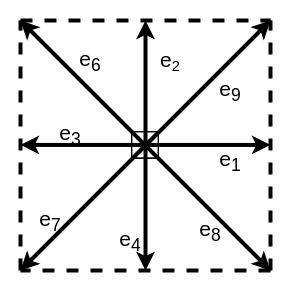
\includegraphics[width=0.5\textwidth]{figures/nine_direction.jpg}
       \caption{A lattice in D2Q9 model and its nine discrete velocities}
       \label{fig:d2q9}
\end{figure}

\begin{equation}
\label{equ:d2q9}
    \overrightarrow{e}_{i} = \left\{\begin{matrix}
(0,0) \qquad\qquad\qquad\qquad\qquad\qquad &i=0 \\ 
(1,0), (0,1), (-1,0), (0,-1)\quad\qquad &i=1,2,3,4 \\ 
(1,1), (-1,1), (-1,-1), (1,1)\qquad & i=5,6,7,8
\end{matrix}\right.
\end{equation}

For each lattice, the distribution function can be thought of as a measure of the probability that the fluid at given position $\mathbf{x}$ has velocity $\mathbf{e}_i$ at time $t$.

As introduced above, in lattice Boltzmann method, the behaviour has been described as the streaming and collision step which are given by Equation~\ref{equ:lbmequ}. In this equation, $fi$ is the distribution function in the direction i; $a$ is the acceleration (given by the external force $F=ma$); $\tau$ is the relaxation time; $f_i^{eq}$ is the equilibrium distribution function in the direction i; $t$ and $\triangle t$ is the time and the increment of time.

\begin{equation}
\label{equ:lbmequ}
f_i(\vec{a}+c\vec{e_i}\triangle t, t+\triangle t) - f_i(\vec x,t)) = \frac{f_i(\vec x, t) - f_i^{eq}(\vec x , t)}{\tau}
\end{equation}



% KS: EXPLAIN ALL SYMBOLS WHEN THEY ARE FIRST INTRODUCED!

In Equation~\ref{equ:lbmequ}, in the left of the equal sign stand for the streaming step and the collision step is in the right. In the actual implementation of our lattice Boltzmann method, we will calculate them separately. The Fig.~\ref{fig:stream} shows how the streaming step exchange its discrete probability distribution.


\begin{figure}[!tb]
   \centering
       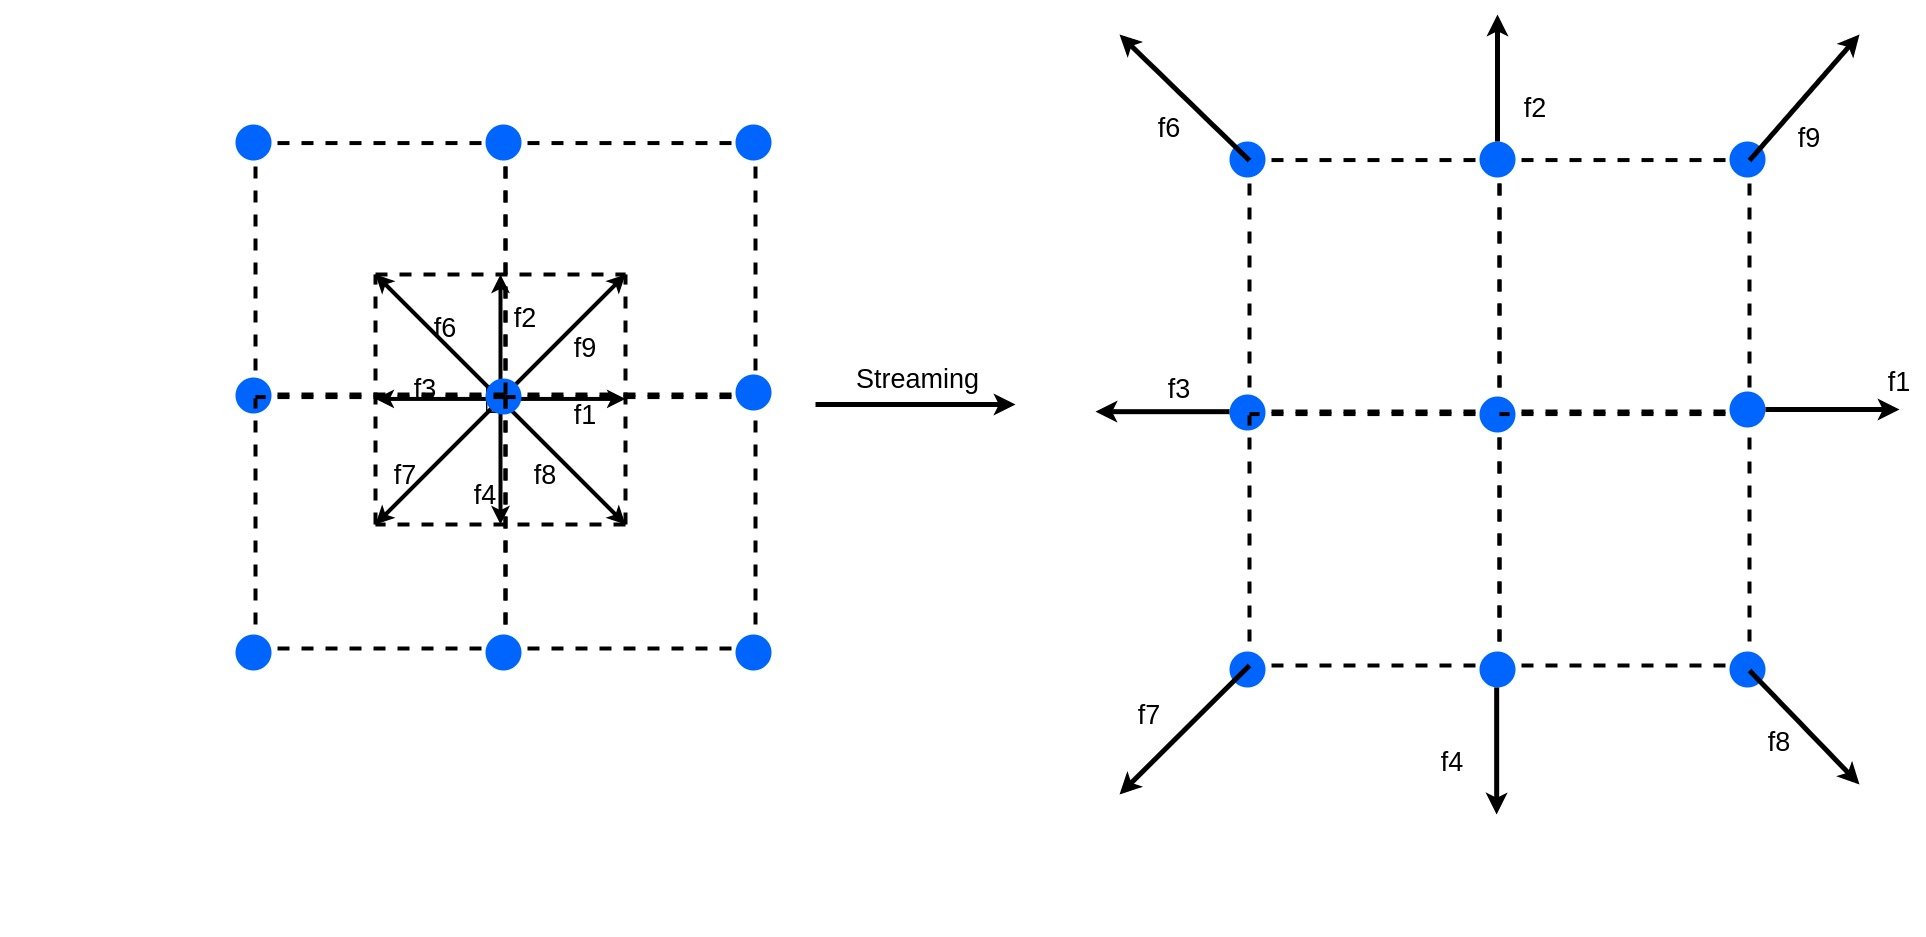
\includegraphics[width=1\textwidth]{figures/stream.jpg}
       \caption{The streaming step of a lattice in D2Q9 model}
       \label{fig:stream}
\end{figure}

In the collision step, Bhatnagar-Gross-Krook (BGK)\ref{sec:BKG} approximation is applied to model the process of relaxation to equilibrium. Qian et al represent the equilibrium distribution function in their the DdQm models as Equation~\ref{equ:collision}. Macro density $\rho$, velocity $u$, weighting factor $w_i$ and lattice speed $c$ are introduced to this process in Equation~\ref{equ:collision}:

\begin{equation}
\label{equ:collision}
    f_i^{eq}(\vec x, t) = \omega_i \rho + \rho w_i \left [  \frac{\vec{e_i}\cdot \vec u}{c^2} + \frac{(\vec{e_i}\cdot\vec u)^2 }{ 2 \cdot c^4 }-\frac{\vec u \cdot \vec u}{2 \cdot c^2} \right ]
\end{equation}

According to Qian et al.'s model of D2Q9, $\omega_i$ is given as:
\begin{equation}
    \omega_i = \left\{\begin{matrix}
4/9 & i=0\\ 
1/9&\quad \quad i=1,2,3,4\\ 
1/36&\quad \quad i=5,6,7,8 
\end{matrix}\right.
\end{equation}

Macroscopic fluid density $\rho (\vec x, t)$ is defined in this model by Equation~\ref{equ:rho}:
\begin{equation}
\label{equ:rho}
    \rho (\vec x, t) = \sum_{i=0}^{8} f_i(\vec x,t)
\end{equation}

Macroscopic velocity $\vec u(\vec x, t)$ is defined in this model by Equation~\ref{equ:u}:
\begin{equation}
\label{equ:u}
    \vec u (\vec x, t) = \frac{1}{\rho} \sum_{i=0}^{8}cf_i\vec{e_i}
\end{equation}

After all, we can summarize the algorithm as follow:
\begin{itemize}
  \item [1] Initialize macroscopic fluid density$\rho$, macroscopic velocity $\vec u$, and discrete probability distribution function $f_i^{eq}$;
  \item [2] Compute the $\rho$, $\vec u$ with Equation~\ref{equ:rho} and Equation~\ref{equ:u};
  \item [3] Compute the equilibrium distribution $f^{eq}_i$ with Equation~\ref{equ:collision};
  \item [4] Collision Step: Update the distribution function $f_i$;
  \item [5] Streaming Step: move $f_i$ to the $f_i^*$ in all nine direction with regarding to $\vec{e_i}$
\end{itemize}


With different initial parameters, the lattice Boltzmann method can simulation different physical problem. As we have discussed in \ref{sec:Obj}, Minion and Brown's problem\cite{minion1997performance} was chosen as a test problem. We will now discuss how to set the initial parameters to assure we are discuss a same physical problem.

% KS: WHAT INITIAL PARAMETERS DO YOU HAVE? 

\subsection{Initial Parameter}
To assure that the implementation is simulating the Minion and Brown's problem\cite{minion1997performance}, we need a criteria. In this case, the Reynolds number can be the criteria. The Reynolds number is the ratio of inertial forces to viscous forces within a fluid which is subjected to relative internal movement due to different fluid velocities\cite{munson2013fluid}. It is used to measure the similitude between fluid dynamics. If we set our parameters to have the same Reynolds number as the case in Minion and Brown's problem, we can assure that we are simulating their problem. In the definition of the Reynolds number at Equation~\ref{equ:neynolds}, $U$ is the velocity, $L$ the length scale, and $nu$ is the kinematic viscosity.
\begin{equation}
\label{equ:neynolds}
    Re = \frac{U \cdot L}{nu}
\end{equation}

In the Minion and Brown's problem, the initial velocity $u$ is defined as Equation~\ref{equ:init_u}, where $k$ is the shear layer thickness; $x$ and $y$ are the position in the system ; $\delta$ is a velocity. 

\begin{equation}
\label{equ:init_u}
    \begin{matrix}
u = tanh(k (y-0.25)) & y \leqslant 0.5 \\ 
u = tanh(k (0.75-y)) & y > 0.5  \\
v = \delta sin(2\pi x )
\end{matrix}
\end{equation}

\begin{figure}[!tb]
   \centering
       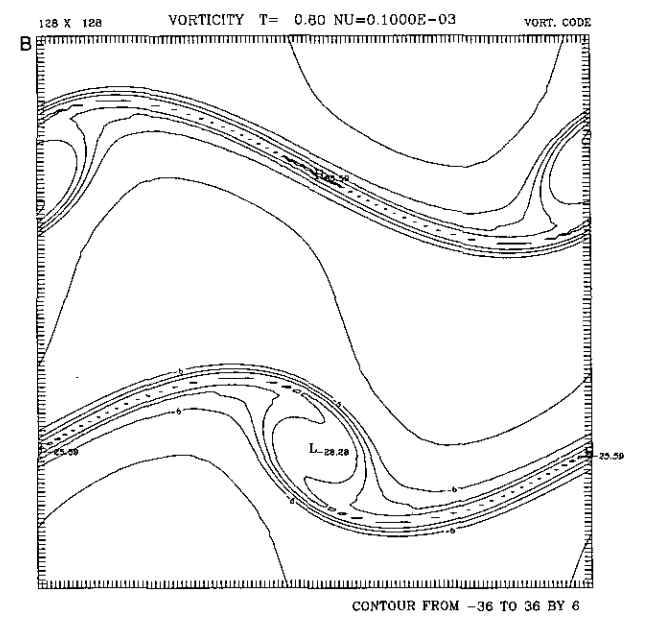
\includegraphics[width=0.8\textwidth]{figures/minion.png}
       \caption{Vorticity contour of the Minion and Brown's work for resolution 128 $\times$ 128. Layer width parameter $\rho = 30$, viscosity $v=1/10,000$, (image from \cite{minion1997performance})}
       \label{fig:minion}
\end{figure}
In the parameters setting in Fig. 4 of Minion and Brown's work (seen Fig.~\ref{fig:minion}), there is a square system with a scale as $L_x = L_y = 1 unit = L$. The shear layer thickness $k$ they used is 30unit. Kinematic viscosity $nu$ is $10^{-4}$. If we take $U = U_0 delta = 0.05$, nu = $10^{-4}$, and $L = 1$, then the corresponding Reynolds number is According to Equation~\ref{equ:neynolds}, we get the corresponding Reynolds number being 500, at Equation~\ref{Re_minion}:
\begin{equation}
\label{Re_minion}
    Re = UL / nu = 0.05 x 1 / 10^{-4} = 500
\end{equation}

After calculate the Reynolds number of the Minion and Brown's work. We can adjust the initial parameters making the Reynolds the same in our implementation. Here, we set the simulation as $L_x = L_y = 128 = L$. The grid space is always $h = 1 unit$. The We now can apply the same initial velocities as Equation~\ref{equ:init_u_lbm}:

\begin{equation}
\label{equ:init_u_lbm}
    \begin{matrix}
u = U_0tanh(k (y-0.25L)) & y \leqslant 0.5 \\ 
u = U_0tanh(k (0.75L-y)) & y > 0.5  \\
v = \delta sin(2\pi x )
\end{matrix}
\end{equation}

Here, we should choose an equivalent value of shear layer thickness $k$; and, according to lattice Boltzmann method, the velocity unit $U_0$ should be less than the speed of sound $c_s$ and we choose $U_0 = 0.01$. To keep the Reynolds number the same, we can get the kinematic viscosity $nu$ being 0.000128 by Equation~\ref{equ:nu_lbm}.

\begin{equation}
    \label{equ:nu_lbm}
    nu = \frac{UL}{Re} = \frac{0.0005 \times 128}{500}  
\end{equation}

Finally, according to Minion and Brown's work, when T=0.8, there is a turbulence in the simulation; see Fig.~\ref{fig:minion}. We can calculate the time step (dimensionless time) by Equation\ref{timestep}. Substitute data from Minion and Brown's setting: time T = 0.8;  unit space $h=1/L=1/128$; unit velocity $U_0 \delta=U=0.05$  into the Equation\ref{timestep}, we know that in this system it need 2000 dimensionless time for the turbulence.

\begin{equation}
\label{timestep}
    T_{step} = \frac{T h}{U_0 \delta} = \frac{0.8 \times \frac{1}{128}}{0.005 } = 5.12
\end{equation}

In the lattice Boltzmann, we have unit space $h=1$, unit velocity $U_0 \delta = U = 0.0005$. Thus, substitute data into Equation~\ref{timestep}, we get $T_{step} = 2000 (timesteps)$, which means for every dimensionless time unit in Minion and Brown's system, we need 2000 steps to simulate to the same progress. In other words, to witness a turbulence in the lattice Boltzmann system, we need at least $5.12 \times 2000 = 10240$ steps. In the implementation and performance evaluation, we used 12000 steps as a standard.\\

A more detailed initialization in serial C used for this project is at Appendix \ref{app:a}.


\vspace*{+3.2cm}
Having covered all the background material needed, we can now review the implementations that constitute one of the contributions of this project.


\newpage


\newpage
\section{Design and Implementation} \label{sec:dai}
This section will be discussing the main contribution of this project: a implementation of lattice Boltzmann method on SpiNNaker.  \\

All the source code is available at: \cite{spinn_lb}
\subsection{Implementation Overview}

As we discussed at \ref{sec:sdw}, in general, SpiNNaker development workflow, the first thing we did is to define the computation graph in Python. We will discuss how we define the lattice vertex (\ref{sec:tlc}), how we define our edge (\ref{sec:tle}), and how we connect them together as a graph (\ref{sec:tcg}). All these steps are implemented in the Python API.
1       
Then on the computation side, as discussed at \ref{sec:lbmb}, there are five steps for a lattice Boltzmann method in general. While the first four steps do not involve communication and can be calculated locally for each lattice vertex (discussed at \ref{sec:cp}), the last step, the streaming step, is where the communication happens, which we will focus on at \ref{sec:ssc}. These computation-wise codes are written in C.

\subsection{The Lattice Cell} \label{sec:tlc}
In this subsection, we will discuss how we design and implement the most basic component with the SpiNNaker GraphFrontEnd, the lattice basic cell.
\subsubsection{Design Consideration} \label{sec:tlcdc}
In the lattice cell class, we will define the data regions needed for simulation. In the implementation, it needs to acquire those data, reserve memory for the data and pass the data in SpiNNaker SDRAM in Python, then define how to read the data from the SDRAM during simulation in C. The data regions that a lattice might need for simulation are: \\

\begin{itemize}
    \item \textbf{System Information:} for every simulation, they at least need some memory reserved for the runtime system such as the how long is a machine time step. And the developers need to generate the system data region and allocate memory for them manually.
    
    \item \textbf{Transmission Information:} for non-embarrassingly parallel problems, the simulation is involved in communication. The keys are generated at runtime, and the developers can ask the mapping system for a fixed number of keys for every lattice. Then the mapping system would allocate continuous keys for the lattice, and the developers would get the base keys of them. The developers can apply for memory for the transmission keys and pass the keys to the cores, correspondingly.

    \item \textbf{Position Information:} in lattice Boltzmann, a lattice might need to know what is its position \textbf{(x,y)} among the whole simulation lattices. The position information would be generated when connecting the lattices as a graph and then pass them into the application.
    
    \item \textbf{Initialized Velocity:} in lattice Boltzmann method, the velocity needs to be generated according to the specific problem. We can either initialize it in Python then pass then in or initialize it in the simulation according to the position. A more detailed discussion is at \ref{sec:ip}.
    
    \item \textbf{Routing Information of Neighbours:} in lattice Boltzmann method, the lattice need to exchange the momentum and energy by moving the distribution function with its eight neighbours. This involves a few communication and the lattice need to know which are its eight neighbours and their routing information, i.e. routing keys to communicate with them. Thus allocating memory and pass them into the cores is necessary. 
    
    \item \textbf{Index of this Lattice:} we might need to know the index of the lattice in the whole simulation fabric. This might not be necessary for a simple prototype. The index of the lattice can be used as a timer delay to avoid communication traffic. We will discuss the communication at \ref{sec:ssc}.
    
    \item \textbf{Result Recording:} the SDRAM in SpiNNaker is relatively limited (\ref{sec:sa}). We can use the recorded data to store larger simulation result more reliably. We can tell the tools how much data per time step and the tools will determine the configuration to keep the SDRAM usage optimal.
\end{itemize}

\subsubsection{Final Implementation}
In the final implementation, we defined the discussed data regions in the \textit{LatticeBasicCell} class following the pattern: get the data; allocate memory; write the data in, where the first step is defined by the developer and the latter two steps are written in Python scripts, and the tool will interpret the scripts to do the actual work. For different data, there are different way to get the data:

\begin{itemize}
    \item \textbf{System Information:} the \textit{SpiNNaker GraphFrontEnd} provide API to generate the system data region.
    \item \textbf{Transmission Information:} the SpiNNaker runtime would allocate keys for the cores.
    \item \textbf{Position Information:} the position information is decided during runtime. it will be passed as class variables.
    \item \textbf{Initialized Velocity:} the velocities are decided during runtime with an initialization function. They will be passed as class variables. 
    \item \textbf{Routing Information of Neighbours:} a lattice can know the which are its neighbours by asking the connected edges. We will illustrate how we implement it at \ref{sec:tle}. After knowing its neighbours, we can get their routing keys via the get\_routing\_info\_from\_pre\_vertex() function from the \textbf{PACMAN} library.
    \item \textbf{Index of Lattice:} we can ask the graph system for the index of a lattice.
    \item \textbf{Result Recording:} we do not need to get data from result recording since it is for the result.
\end{itemize}

After all the data are acquired, we get then reserve corresponding memory and write the data into the SDRAM of each SpiNNaker core; see the upper part of Fig.~\ref{fig:write_data}. Correspondingly, in the C file, we also need to read the data from the SDRAM before the simulation; see the bottom part of Fig.\ref{fig:write_data}. The Fig.~\ref{fig:write_data} shows how we reserve memory for the different data regions and write the data into the SDRAM followed by how to read the written data from the SDRAM during runtime in C.\\
\begin{figure}[tb]
   \centering
       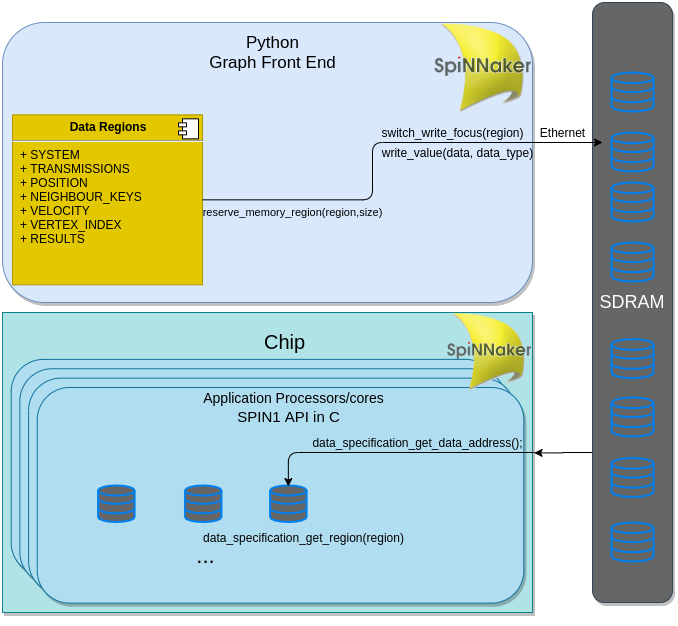
\includegraphics[width=1\textwidth]{figures/write_data.png}
       \caption{The diagram of the implementation of the lattice cell and data specification. In the lattice cell, we define the data regions in Python and the SpiNNaker runtime will interpret our scripts and reserve corresponding memory. In C source file, the lattice cell would read the data from the SDRAM before the simulation.}
       \label{fig:write_data}
\end{figure}



\subsection{The Lattice Edge} \label{sec:tle}
\subsubsection{Design Consideration}
The major job of the lattice edge except connecting two lattice cells is providing a way that the lattice cell can get the vertex on the other end of this edge in a given direction. So that each lattice can get the routing information (routing keys) of its eight neighbours with knowing the direction. \\
\subsubsection{Final Implementation}
In the implementation, the \textit{Lattice Edge class} inherit from the \textit{MachineEdge}, which provided a way to record the pre-vertex and post-vertex, from the \textbf{PACMAN} library. Then we introduced another attribute, \textbf{compass}, to record the relative position of the pre-vertex; see Fig.~\ref{fig:edge}.\\
\begin{figure}[tb]
   \centering
       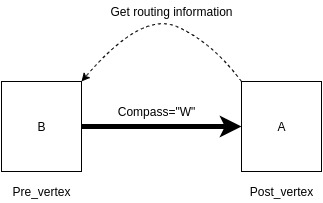
\includegraphics[width=0.7\textwidth]{figures/edge.jpg}
       \caption{A lattice cell A connected by another lattice B via a lattice edge with the compass being "W". The lattice A then can get the routing key from its pre\_vertex, B.}
       \label{fig:edge}
\end{figure}

\subsection{The Computational Graph} \label{sec:tcg} 
\subsubsection{Design Consideration}
In the selected test problem from Minion and Brown\cite{minion1997performance}, the boundary condition we applied for this project is a periodic condition. In the C implementation, we implemented the periodic condition is halo-swapping; see Fig.~\ref{fig:haloswap}. The periodic condition is explicitly applied to the post-collision distribution function $f_i^{*}$ in the streaming step, which introduced extra memory consumption and complexity into the development.\\

Fortunately, in SpiNNaker, the developers do not implement the halo-swapping to apply to the periodic condition explicitly. Instead, SpiNNaker developers can simply connect the lattices on one fringe to the lattices on the opposite fringe via the implemented \textit{Lattice Edge}; see Fig.~\ref{fig:spinnaker_halo}.\\


\begin{figure}[htbp]

\begin{subfigure}[b]{1\textwidth}
       \centering
       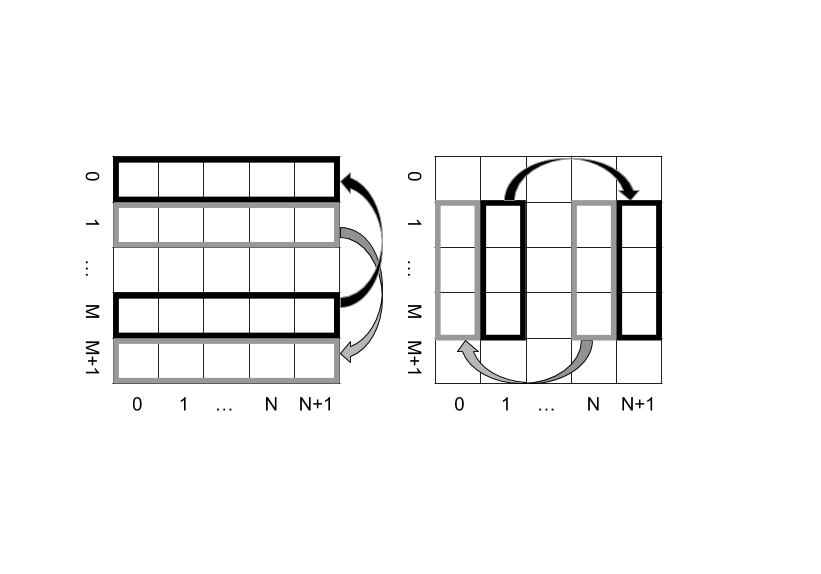
\includegraphics[width=0.8\textwidth]{figures/haloswap.png}
       \caption{A periodic condition in M$\times$N lattice Boltzmann implemented by halo-swapping. We apply this method in our serial C implementation.}
       \label{fig:haloswap}
   \end{subfigure}
   \begin{subfigure}[b]{1\textwidth}
       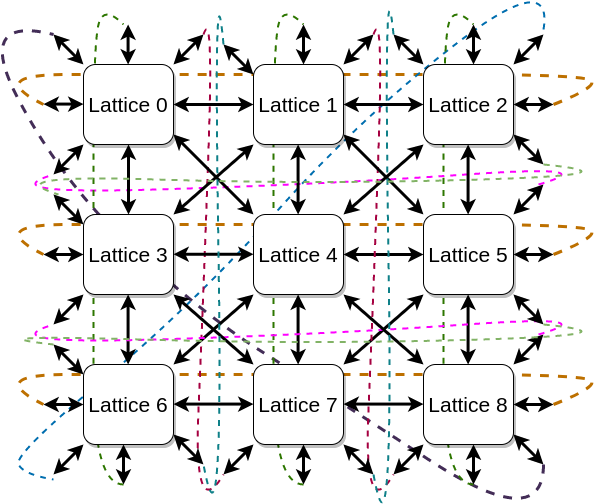
\includegraphics[width=\textwidth]{figures/2dfabric.png}
       \caption{A periodic condition in 3$\times$3 lattice Boltzmann implemented by connecting the lattice periodically via lattice edge. We apply this method in the SpiNNaker implementation.}
       \label{fig:spinnaker_halo}
   \end{subfigure}
   \caption{How we implement a periodic condition in C (\ref{fig:haloswap}) via halo-swap and in SpiNNaker (\ref{fig:spinnaker_halo}) via SpiNNaker graph edge.}
\end{figure}

\subsubsection{Final Implementation}
As we designed, to implement a periodic condition, we connect the lattice cells periodically via lattice edge; see Algo.~\ref{algo:periodic}.\\

\begin{algorithm}
 \caption{The Algorithm to connect the lattice with a periodic condition}
 \label{algo:periodic}
 \KwData{Scale in x dimension: X; Scale in y dimension: Y}
 \SetKwFunction{Connect:}{connect two lattice via a lattice edge}
 \For{i in 0...X}{
    \For {j in 0...Y} {
       Connect Lattice(i,j) with Lattice(i,(j + 1) mod Y)\;
       Connect Lattice(i,j) with Lattice((i + 1) mod X,(j + 1) mod Y)\;
       Connect Lattice(i,j) with Lattice((i+1) mod X, j)\;
       Connect Lattice(i,j) with Lattice((i+1) mod X, (j-1) mod Y)\;
       Connect Lattice(i,j) with Lattice(i, (j-1) mod Y)\;
       Connect Lattice(i,j) with Lattice((i-1) mod X, (j-1) mod Y)\;
       Connect Lattice(i,j) with Lattice((i-1) mod X, j)\;
       Connect Lattice(i,j) with Lattice((i-1) mod X,  (j+1) mod Y)\;
    }
 }
\end{algorithm}




\subsection{Initialize Parameters} \label{sec:ip}
In this subsection, we will discuss how we consider the two different ways to initialize parameters, how we decide and how we implement.\\
\subsubsection{Design Consideration}
To initialize the parameters for the lattice Boltzmann, there are two different ways in general. The first one is initialization on the host (in Python) then passing the initialized parameters into the simulation, and the other one is initialization on SpiNNaker (in C).\\

When initializing parameters in Python on the host, we need to compute the parameters in serial nested loops before the SpiNNaker actually run the simulation. On contrast. If we are initializing the parameters in SpiNNaker, the parameters would be computed distributively on each individual core. Besides, vanilla Python is commonly regarded as being poor in scientific computing, especially in nested loop.\\

It is reasonable that initialization in C on the simulation runtime would be faster in speed comparing with initialization in Python in serial. Thus, our first implementation was based on C and computed the initial parameters distributively on each core. \\

However, there are two points that we do not take into consideration when it comes to the real implementation on SpiNNaker. The first one is that, as we introduced before \ref{sec:ca}, SpiNNaker is using ARM968 cores which have no floating-point hardware, and we have to use fixed-point arithmetic or software-based floating-point arithmetic. It introduced some challenges in using the mathematical library in C, including \textbf{math.h}. The other one is that, as we also introduced before \ref{sec:ca}, the SpiNNaker cores have relatively limited ITCM (instruction tight-coupled memory). If we use the mathematical library such as \textbf{math.h}, the bloated math library will run out of the limited ITCM. Although it is possible to implement mathematics functions such as \textbf{tanh} by applying the Taylor series, the accuracy and efficiency of the hand-write functions do not satisfy the requirements of this simulation.\\

After carefully reconsidering the whole process, we finally decided to implement the initialization on the host in Python and then write the initialized parameters as data regions into the SpiNNaker device. \\
\subsubsection{Final Implementation}
we had implemented the initialization function in C for the serial version; see Appendix.~\ref{app:a}. It uses two-level nested-loop to initialize the velocities and the macroscopic densities for every actual lattice according to the settings of the test problem. Here the actual lattices are those which sit in the inner part of the simulation and the outermost layer would be used as halo-swapping.\\

For SpiNNaker version, since we have to instantiate the LatticeBasicCell class and the initialized parameters need to be passed as attributes during the instantiation, instead of calculating the parameters of all lattices at once, we calculate the parameters every time before a lattice being created. Then when the lattices are created, the parameters are initialized as well.\\

In the implementation of the SpiNNaker version of LBM, we implement the initialization of velocity function in Python and pass the result as attributes before the instantiation. For the macroscopic density, since we are setting all the initial macroscopic densities $\rho$ as 1.0, we can directly initialize them in the C source file.  \\

\subsection{Computation Implementation} \label{sec:cp}
This subsection will discuss how we design and implement the behaviours except inter-core communication of a lattice.\\
\subsubsection{Design Consideration}
The computation part of the simulation is the process that does not involve communication. According to the five steps of a lattice Boltzmann method in \ref{sec:lbmb}, we can draw the algorithm for each individual lattice; see Algo.~\ref{algo:lbm}.\\

\begin{algorithm}
 \caption{The Algorithm of the lattice Boltzmann method for a individual lattice.}
 \label{algo:lbm}
 Initialize\;
 \While {not finish} {
  compute $\rho$ and $\vec u$\;
 compute $f_i^{eq}$\;
 \tcc{Collision Step}
 collideStep: Move $f_i$ to $f^*$ \;  
  \tcc {Streaming step start}
 Send $f_i$ to its neighbours\;  
 Receive neighbours' $f_i$ as $f_i^{*}$\; 
 \tcc {Streaming step end}
 }
 
\end{algorithm}

From the Algo.~\ref{algo:lbm}, we can see that the algorithm except the streaming steps do not need any inter-core communication, and those computations can be done distributively by each individual core.\\

\subsubsection{Final Implementation}
For the actual implementation, we need to take SpiNNaker's features into account. In this project, we use the time ticker provided by SpiNNaker as a trigger for each iteration instead of directly execute the loops. The reason why we choose this method is that it provides an easier way to manage the communication, which we will discuss in \ref{sec:co}.\\

\begin{figure}[!tb]
   \centering
       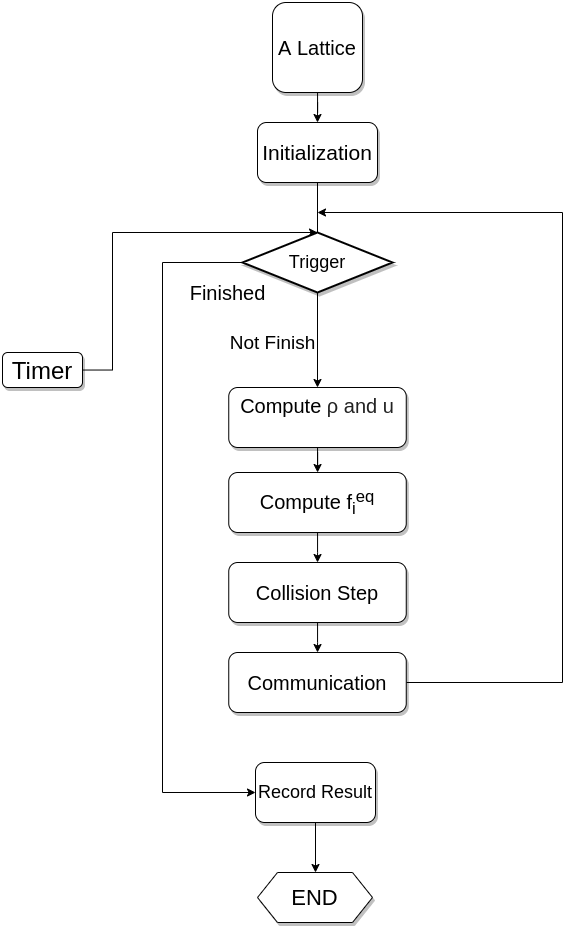
\includegraphics[width=0.6\textwidth]{figures/computation.png}
       \caption{A diagram of the computation processes of a Lattice. After initialization, the lattice starts the simulation. The built-in timer will send a timer tick for every a fixed time, and the time tick would trigger the simulation for the next time step until the simulation ends. In this case, we do not take the communication into consideration.}
       \label{fig:computation}
\end{figure}

As Fig.~\ref{fig:computation} shows, the after the initialization, whenever the lattice receive a time tick and the simulation is not ending, it will run another computation loop. After all, simulations completed at this core, it will record the result to the buffer and change its state as ready for the front end extracting the buffer.\\

\subsection{Communication Implementation} \label{sec:ssc}
As we discussed above, the only part of LBM that involve communication is the streaming step. Therefore, in this subsection, we will discuss how we design the steaming step of the lattice and how we implement sending the multicast packets and acquired the data.\\
\subsubsection{Design Consideration}
Firstly, we need to consider what data we need to seed via multicast. In the steaming step of the lattice Boltzmann method, the post-distribution functions $f_i^*$ in nine directions are the distribution function of its neighbours in the corresponding directions. In this case, for each individual lattice, since it is itself in the first direction, it need to send its rest eight distribution functions $f_i$ via multicast; see Fig.~\ref{fig:spinn_send}. In this case, the number of multicast packets is 8.\\

Then we have to consider the multicast packets each lattice need. As we discussed above, each lattice will send eight multicast packets from each of its neighbours. Therefore, the total multicast packets a lattice need to acquire is $8 \times 8 = 64$; see Fig.~\ref{fig:spinn_receive}.\\

\begin{figure}[!tb]

\begin{subfigure}[!tb]{0.5\textwidth}
       \centering
       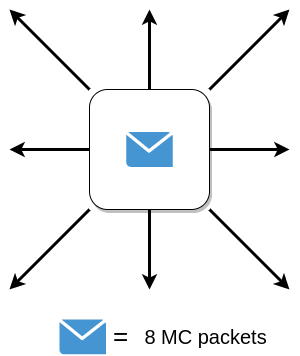
\includegraphics[width=0.5\textwidth]{figures/send.png}
       \caption{A lattice send its distribution function $f_i$ in 8 directions via SpiNNaker multicast. For every streaming step, the lattice will send 8 multicast packets.}
       \label{fig:spinn_send}
   \end{subfigure}
   \begin{subfigure}[!tb]{0.5\textwidth}
   \centering
       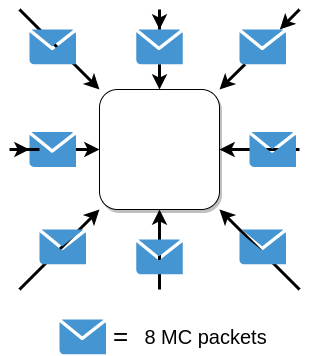
\includegraphics[width=0.5\textwidth]{figures/receive.png}
       \caption{A lattice acquire the distribution function of its 8 neighbours from multicast packets as it post distribution function $f_i^{*}$. For every streaming step, the lattice will receive $8\times8=64$ packets.}
       \label{fig:spinn_receive}
   \end{subfigure}
   \caption{Tha diagram of communication implementation of LBM on SpiNNaker. On the sender side (a), the lattice need to send the distribution function as 8 multicast packets; on the receiver side (b), the lattice need to collect 64 packets from it neighbours and extract the post-distribution function from the payloads.}
\end{figure}

However, not all 64 multicast packets are necessary for a lattice. From each direction, the lattice only needs the corresponding one distribution function. In other words, the lattice only needs one multicast packet from one direction. Therefore, a lattice only actually need eight multicast packets though it still needs to acquire all 64 packets to know which are eight packets it needs.\\

\subsubsection{Implementation}
In the implementation, the first challenge is that, in SpiNNaker, by default, we can only send 32bit integer via multicast packet, while the numerical format we used in this project is floating-point. Our solution, which is also the commonly used solution in SpiNNaker, is converting the floating-point number to unsigned integer when sending the multicast packets and convert the unsigned integer back to floating-point when reading the payload of multicast packets by using the \textbf{union} structure in C.\\

The second challenge is to recognize where a packet comes from. In the implementation, instead of only adding the payloads of the packets, we add both the key and the payload into the circular buffer. Then we can firstly get the key of the packet knowing the packet coming from which direction then get the corresponding payload.\\

Finally, because SpiNNaker multicast does not guarantee the delivery of packets, to ensure that every lattice receives the correct number of packets, we implement a safety check function to interrupt the program when not all lattice receive the correct number of multicast packets. As we discussed before, for every time step, each lattice should receive 64 packets, where 8 of them is necessary, and 56 of them should also be confirmed as delivered for the sake of safety.\\

In conclusion, as Fig.~\ref{fig:communicate} shows, to implement the steaming step by communication, the lattice will first convert the corresponding distribution function from floating-point to unsigned integer. Then it sends the converted payload with the corresponding key. On the receiver side, it will first store both the key and payload into the circular buffer. When it collects the correct number of buffer (in this case, the correct number of the buffer is $64\times2 = 128$), it will extract key and payload from the buffer. Finally, the receiver will save the convert-backed payload into $f_i^*$ as post-distribution function and the streaming step end.\\
\begin{figure}[!tb]
   \centering
       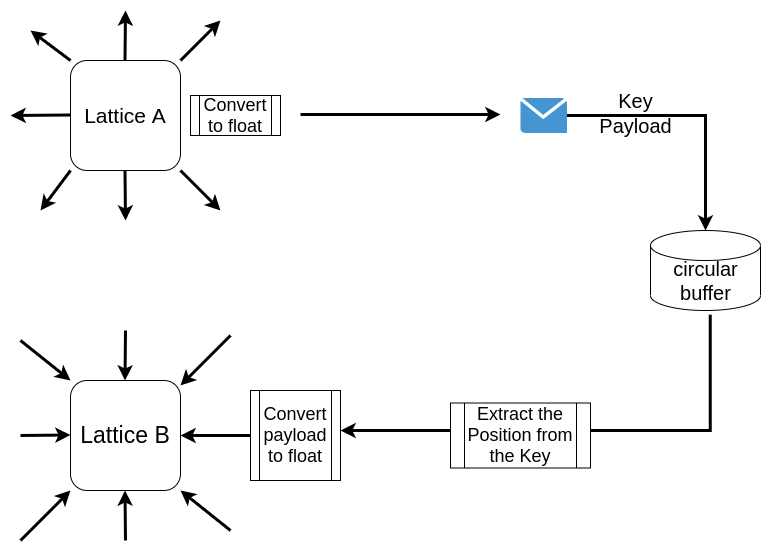
\includegraphics[width=0.8\textwidth]{figures/communication.png}
       \caption{A diagram of the communication process between two adjacent lattices. In this diagram, Lattice A sends a multicast packet, and Lattice B is one of the receivers. Before A sending the MC packets, it firstly converts the distribution function $f_i$ into an integer. Then it sends the converted $f_i$ with the corresponding key. When Lattice B captures the MC packet, it firstly adds the key and payload into the circular buffer. When B capture all the packets for this time step, it stores  the packets of them to $f_i^*$ as post-distribution function.}
       \label{fig:communicate}
\end{figure}

This report up to this point has described how to implement a basic lattice Boltzmann method on SpiNNaker, and it is sufficient for simulation in relatively small simulation (e.g. 32 lattices $\times$ 32 lattices). However, for real-world simulation, the scalability is important. We need to do further optimization for the potential real-world simulation.\\

\subsection{Communication Optimization} \label{sec:co}
In this section, we will first discuss why the basic implementation cannot run large scale simulation in a relatively short time. Then we will introduce how we optimize the communication for the potential larger simulation.\\
\subsubsection{Design Consideration}
As we illustrated before, because there is no guarantee of packet delivery and other issues including back pressure and packets collision will cause packets drop, we introduced a safety check before every time step. The simulation will always pass the safety check when there are only a small number of packets firing in the network when the scale of simulation is relatively small. However, if the simulation scale becomes larger enough, there would be more packets in the network during the same period of time. Although, if there is a dumped packet, the re-injector would have the ability to re-inject. When some unnecessary procedures slowing down the simulation and there are too many packets firing at the same time; see Fig.~\ref{fig:packet_error}, the re-injector might not be able to re-inject and, as a consequence, the simulation will not pass the safety check for the next time step. Eventually, the program would produce a runtime error.\\

\begin{figure}[!tb]
   \centering
       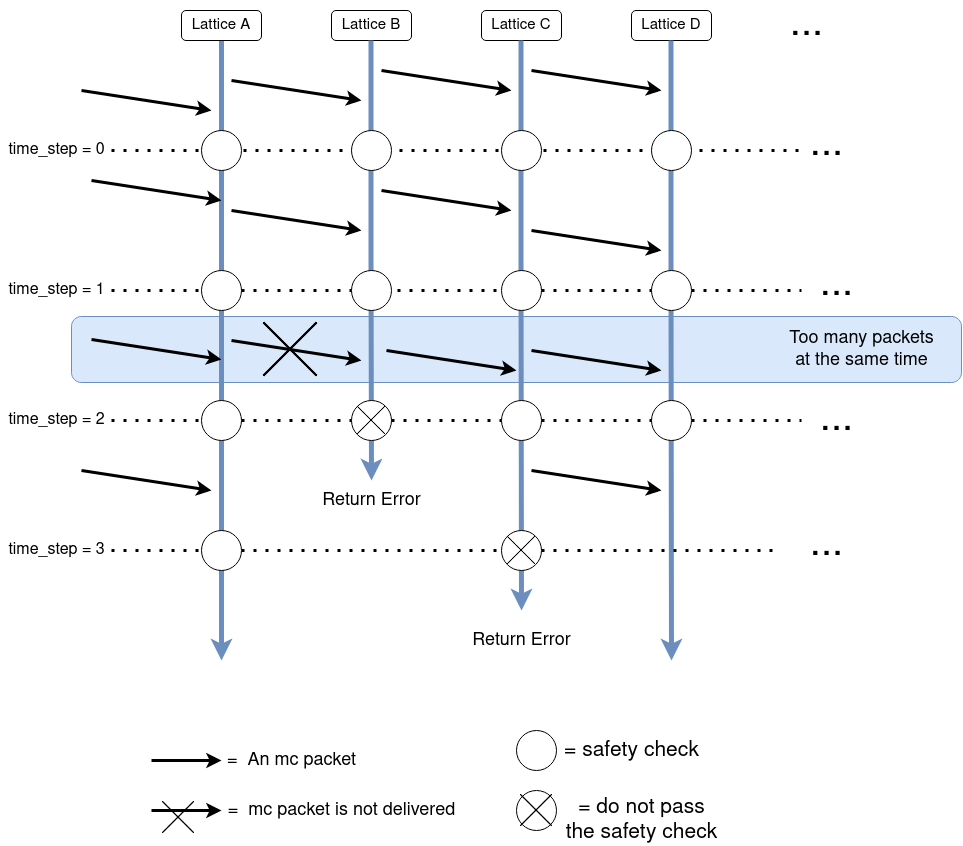
\includegraphics[width=1\textwidth]{figures/packet_error.png}
       \caption{When there are too many packets firing in the network at the same time, it is highly possible that the packets would be dumped. Though the re-injector might be able to re-inject the packets, when there are too many packets need to re-inject and the time is not enough, the lattice (lattice A in this diagram) will not pass the safety check and return a runtime error. The simulation of this core then will stop. The other core will stop because of safety check successively.}
       \label{fig:packet_error}
\end{figure}
\subsubsection{Final Implementation}
In order to address these issues, firstly we remove all unnecessary procedures, i.e. printing log information to the IO buffer and only remain those logs which are essential for debugging.\\

Secondly, to reduce the peak packet rate, we firstly introduced a delay between sending multicast packets. In the implementation, to make the delays of the lattices as different from each other as possible, we add delays based on the index of cores; see Fig.~\ref{fig:packet_offset}. With considering not introduce a too big delay when the scale of simulation is large, after experiments, we finally use Index mod $400$ as the delay between sending.\\

Finally, even though we have made some efforts to reduce the peak packet rate, for an even larger simulation, we need to reduce it even further. Therefore, we further introduce timer offset to further reduce the chance of them sending messages at the same time; see Fig.~\ref{fig:packet_offset}.\\

\begin{figure}[!tb]
   \centering
       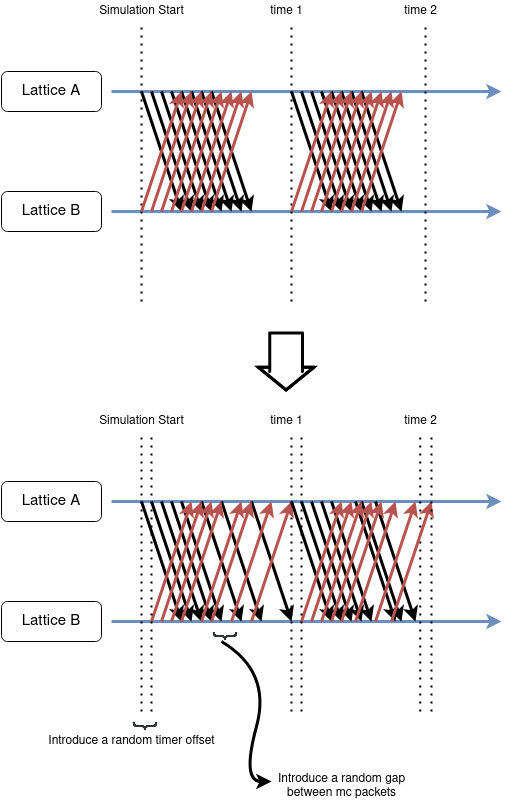
\includegraphics[width=0.8\textwidth]{figures/optimize.png}
       \caption{When there are too many packets firing in the network at the same time, it is highly possible that the packets would be dumped. Though the re-injector might be able to re-inject the packets, when there are too many packets need to re-inject and the time is not enough, the lattice (lattice A in this diagram) will not pass the safety check and return a runtime error. The simulation of this core then will stop. The other core will stop because of safety check successively.}
       \label{fig:packet_offset}
\end{figure}


\newpage
\section{Result and Evaluation} \label{sec:eval}
This section discuss the result of the simulation with our implemented lattice Boltzmann method on SpiNNaker. Firstly, the evaluation setup (\ref{sec:es}) including the serial version and SpiNNaker version would be discussed. Then we will discuss the correctness and the accuracy of simulation in different scale at \ref{sec:caae}. Then we will compare the performance in term of speed with the serial implementation in CPU at \ref{sec:perfe}.
\subsection{Evaluation Setup} \label{sec:es}
In this project, we used a serial implementation of the test problem in C as the baseline. The serial version would be run on EPCC's facility Cirrus (Intel Xeon E5-2695 (Broadwell)), with no compiler optimization.\\

On the SpiNNaker side, we run our simulation on the SpiNNaker cluster in the University of Manchester, which contains 1,036,800 cores via the SpiNNaker Jupyter Notebook interface. \\

For evaluation, we use three different scale of simulation; see \ref{table:setting}. We will firstly plot the contour graph of the result of those three simulation. Those simulation indicate the same problem but in different resolution. Then we will use the normalized distances L-1 norm, L-2 norm and L-infinite norm  of (1) SpiNNaker version vs. Serial float version; (2) SpiNNaker version vs. Serial double version; (3) Serial float version vs. Serial double version to discuss the correctness and the accuracy of our SpiNNaker implementation.\\

\begin{table}[tb]
\centering
\begin{tabular}{|c|c|c|c|}
\hline
Scale          & 64$\times$64 & 128$\times$128 & 256$\times$256 \\ \hline
total cores    & 4086         & 16384          & 65536          \\ \hline
total timestep  & 5120         & 10240          & 20480          \\ \hline
$\nu$           & 0.000064     & 0.000128       & 0.000256       \\ \hline
$\tau$           & 0.500192     & 0.500384       & 0.500735       \\ \hline
\end{tabular}
\caption{The physical parameters setting in three different scales.}
\label{table:setting}
\end{table}


For performance, in this project, we focus on speed. To more visually compare the magnitude of the relationship between them, after confirmed the correctness, we do not take physical settings into consideration. In other words, all the experiments of those three scale would run for 12000 time steps. We will compare the total simulation time and the simulation time per time step of the SpiNNaker implementation and serial implementation in the three scales. \\

It should be noted that, in SpiNNaker, we do not take the time spend on loading SpiNNaker hardware configuration into account for the above comparison. We will discuss it in more detail at \ref{sec:ana}.\\

To make the results more plausible, we took the tie value for three executions for every result.\\
\subsection{Correctness and Accuracy Evaluation} \label{sec:caae}
Firstly, we can get an general judgement on the correctness from the vorticity contour. In Fig.~\ref{fig:contour}, Fig.~\ref{fig:a},Fig.~\ref{fig:c} and Fig.~\ref{fig:e} is produced from the serial C implementation in double floating precise. According to \cite{minion1997performance}, with its configuration, there would be a turbulence in the periodic system. It is clear that there are turbulence in all three scale. Turbulence is recognized as a complex system and if there is any small error during the calculation, eventually, the result would be markedly different. In this case, we got a similar turbulence as \cite{minion1997performance}; and now We are confident enough that our serial implementation is correct.\\

On the left hand side of \ref{fig:contour}, we have the contour result from the SpiNNaker implementation. It is clear that the result from the SpiNNaker implementation has similar contours as the serial C implementation. We can now say that our implementation is correct. However, CFD need accuracy and if we want to know how accurate our simulation is, we need to analysis the result numerically.\\

\begin{figure}[htbp]  
\begin{subfigure}{0.43\textwidth}
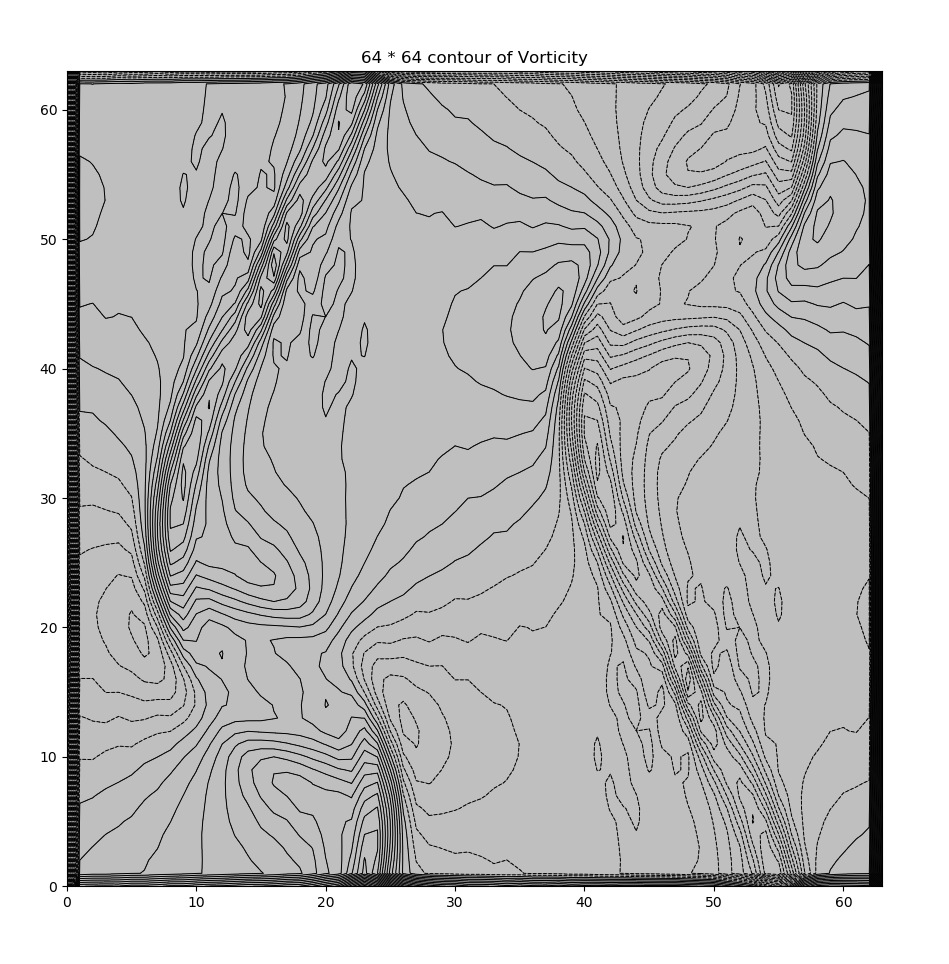
\includegraphics[width=\linewidth]{figures/double_c_64.png}
\caption{Contour of 64$\times$64 from serial C implementation} \label{fig:a}
\end{subfigure}\hspace*{\fill}
\begin{subfigure}{0.57\textwidth}
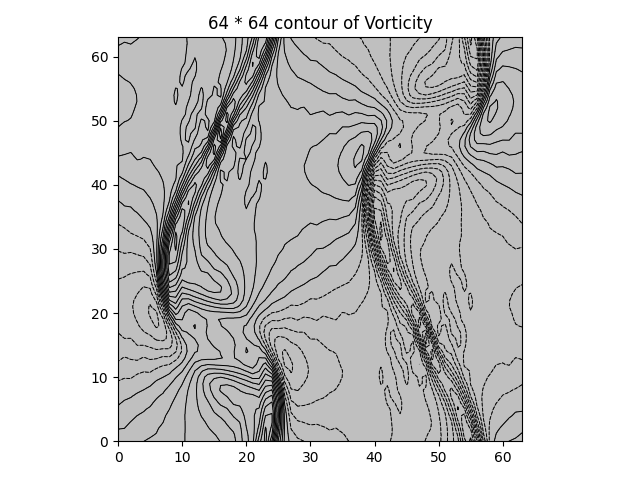
\includegraphics[width=\linewidth]{figures/spinnaker_64.png}
\caption{Contour of 64$\times$64 from SpiNNaker implementation} \label{fig:b}
\end{subfigure}

\medskip
\begin{subfigure}{0.43\textwidth}
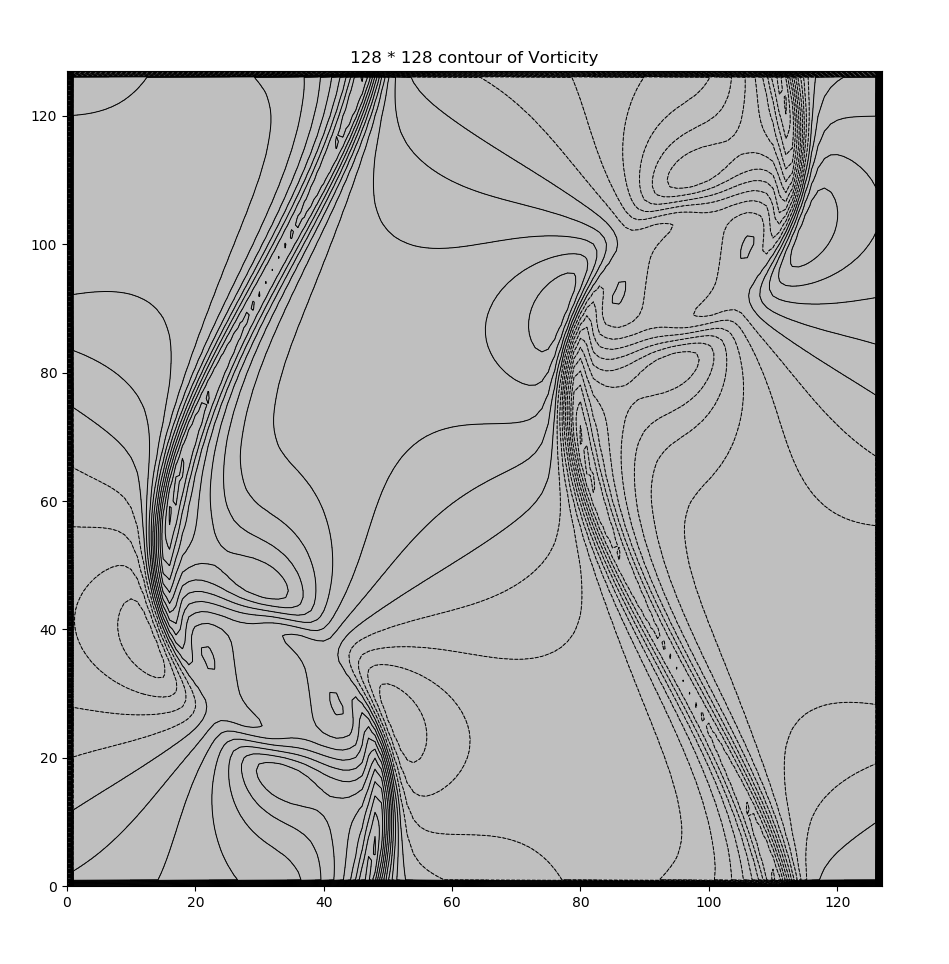
\includegraphics[width=\linewidth]{figures/double_c_128.png}
\caption{Contour of 128$\times$128 from serial C implementation} \label{fig:c}
\end{subfigure}\hspace*{\fill}
\begin{subfigure}{0.57\textwidth}
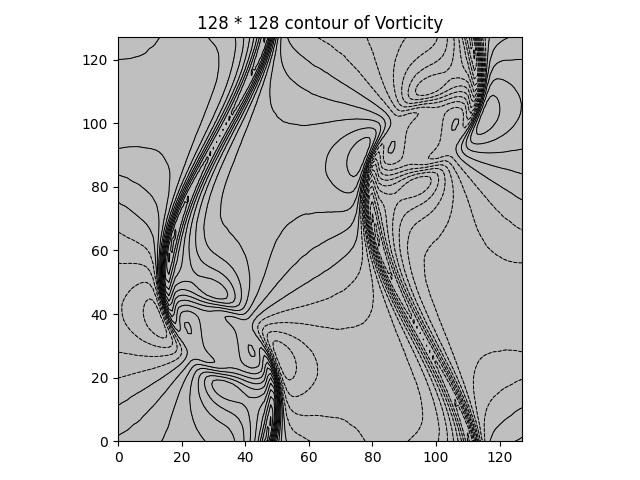
\includegraphics[width=\linewidth]{figures/spinnaker_128.png}
\caption{Contour of 64$\times$64 from SpiNNaker implementation} \label{fig:d}
\end{subfigure}

\medskip
\begin{subfigure}{0.43\textwidth}
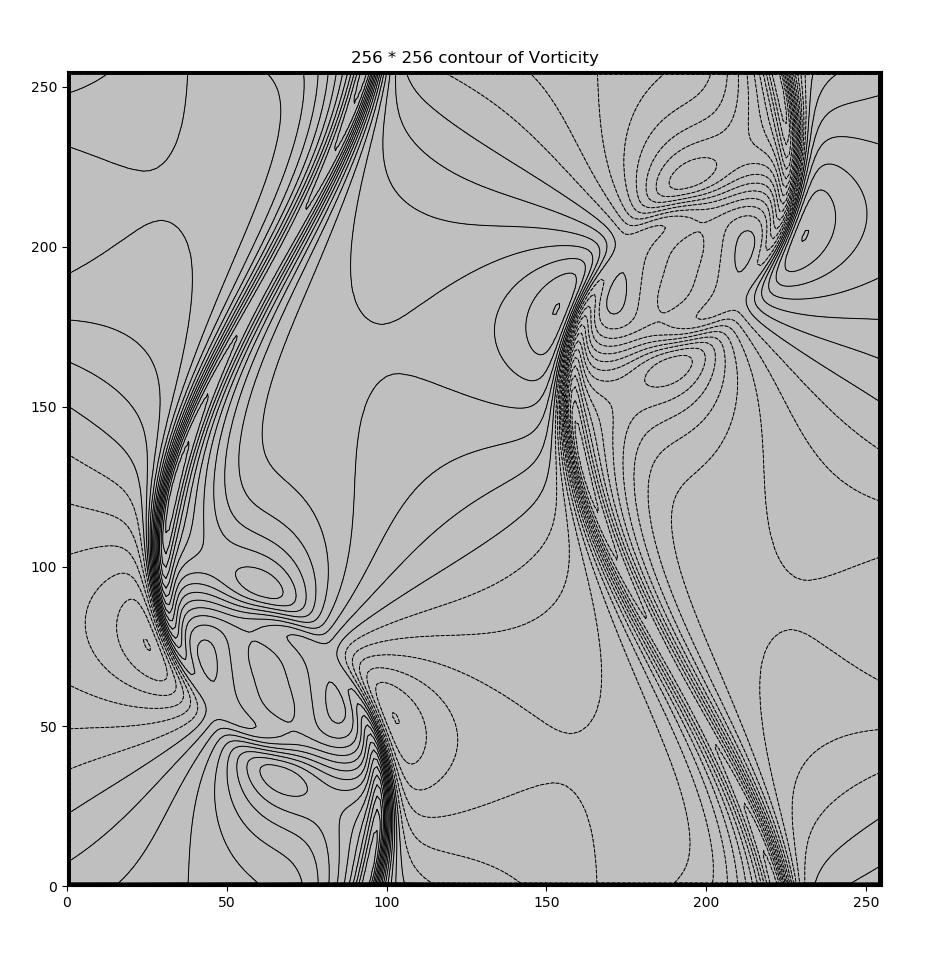
\includegraphics[width=\linewidth]{figures/double_c_256.png}
\caption{Contour of 256$\times$256 from serial C implementation} \label{fig:e}
\end{subfigure}\hspace*{\fill}
\begin{subfigure}{0.57\textwidth}
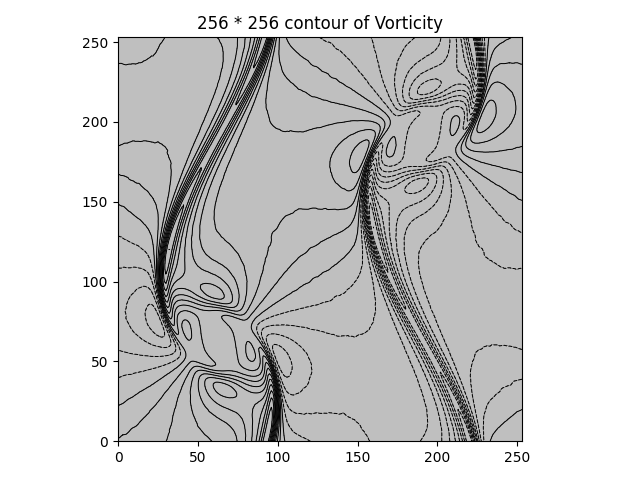
\includegraphics[width=\linewidth]{figures/spinnaker_256.png}
\caption{Contour of 64$\times$64 from SpiNNaker implementation} \label{fig:f}
\end{subfigure}
\caption{Contour graphs of the simulations in three different scale. \ref{fig:a},\ref{fig:c},\ref{fig:e} are the contour graph with scale of $32\times32$, $64\times64$ and $128\times128$ from serial C implementation in double floating precise.\ref{fig:b},\ref{fig:d},\ref{fig:f} are the contour graph with scale of $32\times32$, $64\times64$ and $128\times128$ from SpiNNaker implementation.} 
\label{fig:contour}
\end{figure}

In Table.~\ref{table:norm}, we show how we quantifying the variation between different results. We can regard the double precis serial C version as a baseline and compare it with the floating-point implementation in serial C. From the table, it is clear that in terms of $L-$ norm, $L-2$ norm and $L_{infi}$, SpiNNaker implementation maintained at the same level as C. More specifically, we introduced another criteria, the L-2 norm per grid, to quantify effect of error on each grid; and the L-2 per grid of SpiNNaker implementation also stay at the same level of floating-point C implementation. Therefore, we can confirm that, in terms of accuracy, SpiNNaker's LBM implementation is already at the level of existing CPUs.\\

\begin{table}[tb]
\begin{tabular}{|c|c|c|c|c|}
\hline
Scale                & Norm        & float vs. double& float vs. SpiNNaker& double vs. SpiNNaker\\ \hline
\multirow{4}{*}{64}  & L-1          & 0.003145             & 0.004472              & 0.003632               \\ \cline{2-5} 
                     & L-2          & 6.3365e-05           & 9.133678e-05          & 7.513214e-05           \\ \cline{2-5} 
                     & $L_{infi}$  & 4.2000e-06           & 6.600575e-06          & 5.867303e-06           \\ \cline{2-5} 
                     & L-2 per Grid & 1.54700e-08          & 2.22990e-08           & 1.83428e-08            \\ \hline
\multirow{4}{*}{128} & L-1          & 0.012635             & 0.013630              & 0.015220               \\ \cline{2-5} 
                     & L-2          & 0.000126             & 0.044751              & 0.000152               \\ \cline{2-5} 
                     & $L_{infi}$  & 4.50000e-06          & 4.416680e-06          & 5.739052e-06           \\ \cline{2-5} 
                     & L-2 per Grid & 7.69043e-08          & 2.73138e-06           & 9.27734e-09            \\ \hline
\multirow{4}{*}{256} & L-1          & 0.047357             & 0.056009              & 0.032206               \\ \cline{2-5} 
                     & L-2          & 0.000239             & 0.000278              & 0.000142               \\ \cline{2-5} 
                     & $L_{infi}$  & 4.300000e-06         & 4.80000e-06           & 9.000001e-06           \\ \cline{2-5} 
                     & L-2 per Grid & 1.4296e-08           & 1.7792e-08            & 9.088e-09              \\ \hline
\end{tabular}
\caption{A chart of three different matrix norm between each two of floating-point C, double precis floating-point C and SpiNNaker. Here we use L-1 norm, L-2 norm and L-infinite norm to quantify the extent of variation in results. Besides, we introduce another criteria L-2 norm per grid to quantify the variation of each lattice.}
\label{table:norm}
\end{table}

\subsection{Performance Evaluation} \label{sec:perfe}
After quantifying the correctness and the accuracy, we now have a reasonably correct implementation. Then To make it easier to measure its performance, we execute the simulation with different scale in the same time step i.e. 12000 steps.\\

\begin{figure}[tb]
   \centering
       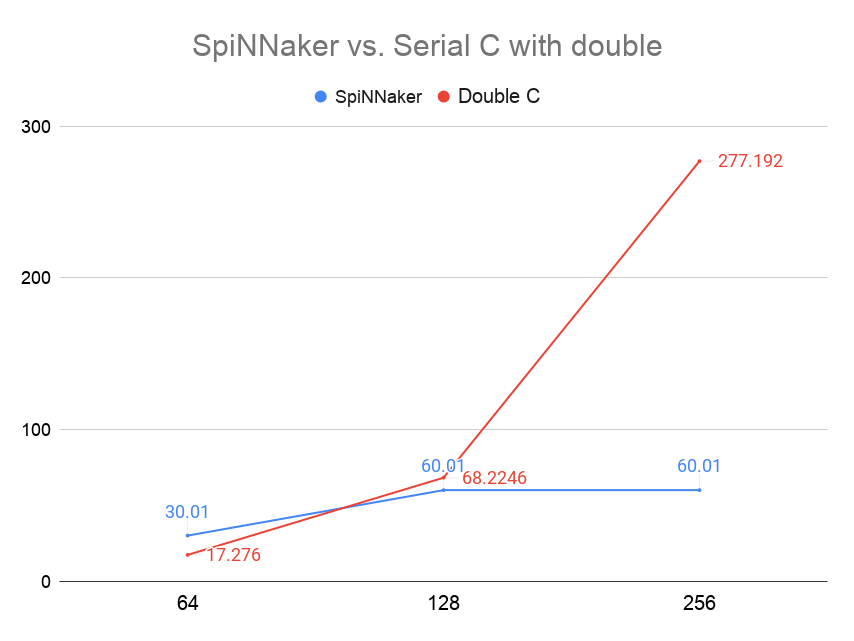
\includegraphics[width=0.8\textwidth]{figures/SpiNNaker vs. Serial C with double.png}
       \caption{Execution time of 12000 time steps in scale of $64\times64$, $128\times128$ and $256\times256$ with SpiNNaker implementation and serial implementation.}
       \label{fig:performance}
\end{figure}

As Fig.~\ref{fig:performance} shows, as the size of the simulation increases, the execution time of the serial program increases rapidly. When the simulation size is small, the serial program executes more efficiently than SpiNNaker; however, as the task size increases, the SpiNNaker naturally implementation utilizes more cores and gets better performance accordingly. For $128\times128$ simulation, the SpiNNaker gain $277.192 / 60.01 = 4.61$ speed-up. With this implementation and hardware, we achieve a relatively good weak-scaling performance.\\

It is noticeable that in SpiNNaker $128\times128$ simulation and $256\times256$ simulation need the same amount of time. This is because: (1) in this project, we only allocate 1 lattice per core. And as the scale of simulation increase, the SpiNNaker implementation will correspondingly increased use of cores; (2) in this project, we have not yet get the optimal performance of SpiNNaker, especially for $128\times128$ simulation. To get a better performance, we are supposed to adjust the SpiNNaker configuration, e.g. timer offset, time scale factor, delay between multicast, really carefully, which need time that beyond the scope of this project.


\subsection{Limitation Analysis} \label{sec:ana}
The first limitation is from the device itself. In the previous performance analysis, we only take the time spend on \textbf{simulation}, which means we do not take the non-simulation time ,e.g. booting the machine, loading data specification to the device, loading data back to host etc., into account. In fact, with the increasing scale of the simulation, the time spend on the non-simulation tasks become larger; see \ref{fig:loading}.

\begin{figure}[tb]
   \centering
       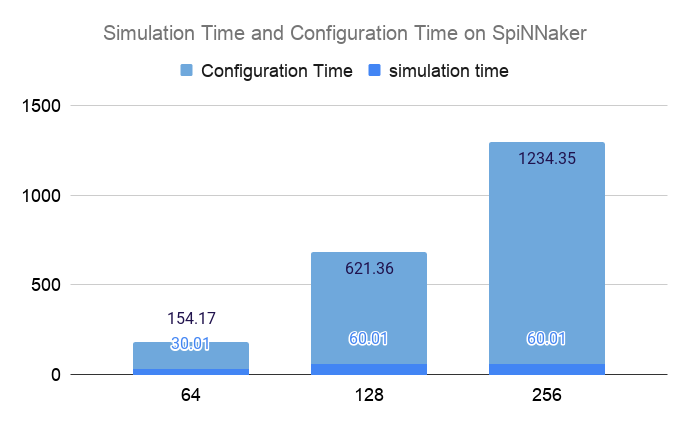
\includegraphics[width=0.8\textwidth]{figures/Simulation Time and Configuration Time on SpiNNaker.png}
       \caption{Simulation time and the configuration time for three different scale simulation. From the chart, it is clear that as the increasing of the simulation scale, there are more time spending on setting up the device and get the simulation result back to host.}
       \label{fig:loading}
\end{figure}

At the moment, it's not possible to solve the problem completely, because as the increasing of simulation scale, there will be more data need to transfer before and after the simulation. However, a group of researchers and engineers are working on tools that enable the SpiNNaker to load data in parallel, which would accelerates data transfer greatly.

Another limitation is that, in this project, we only allocate 1 lattice per SpiNNaker core. Although, we can get parallelism from this configuration, the number of available cores significantly limits the upper limit of simulation scale. In this implementation with available SpiNNaker hardware (about 1,000,000), the maximum scale of simulation is around  $1000 \times 1000$, which is not yet sufficient for real-world engineering problems.
\newpage
\section{Conclusion}
\subsection{Summary}
\subsection{Future Work}






\newpage
\appendix
\section{Appendix - Initialization function in Serial C} \label{app:a}
\begin{minted}{C}
double U_0 = 0.01;
double K = 30.0;
double delta = 0.05;
/*
 * Init the velocity u, v = (u_x, u_y)
 * 
 * ydim = xdim = N = 128
 * K = 30 / N
 * delta = 0.05
 * 
 * u = tanh( K (y - 0.25 * ydim) ) for y <= 0.5 * ydim 
 * u = U_0 tanh( K (0.75 * ydim - y) ) for y >  0.5 * ydim
 * 
 * v = delta sin( 2pi *x / xdim )
*/
void initRho_N_U(double (*u_x)[ydim + 2], double (*u_y)[ydim + 2], double (*rho)[ydim + 2])
{
    for (int i = 1; i < xdim + 1; i++)
    {
        for (int j = 1; j < ydim + 1; j++)
        {
            double x_temp, y_temp;
            x_temp = 1.0 * (double)(i - 1) / (double)xdim;
            y_temp = 1.0 * (double)(j - 1) / (double)ydim; // scale the i and j to make 0 < i,j < 1

            if (y_temp <= 0.5)
            {
                u_x[i][j] = U_0 * tanh(K * (y_temp - 0.25));
            }
            else
            {
                u_x[i][j] = U_0 * tanh(K * (0.75 - y_temp));
            }

            u_y[i][j] = U_0 * delta * sin(2.0 * M_PI * (x_temp + 0.25));
            rho[i][j] = 1.0;
        }
    }
}
\end{minted}
\newpage
\section{Appendix - Initialization function in Serial Python for SpiNNaker} \label{app:b}
\begin{minted}{Python}
ex = [0, 1, 0, -1, 0, 1, -1, -1, 1]
ey = [0, 0, 1, 0, -1, 1, 1, -1, -1]

def initVelocity(x_pos, y_pos):
    """
    Init the velocity u, v = (u_x, u_y)
  
    ydim = xdim = N = 128
    K = 30 / N
    delta = 0.05
  
    u = tanh( K (y - 0.25 * ydim) ) for y <= 0.5 * ydim 
    u = U_0 tanh( K (0.75 * ydim - y) ) for y >  0.5 * ydim
    v = delta sin( 2pi *x / xdim )
    """
    U_0 = 0.01
    K = 30.0
    delta = 0.05
    x_temp = 1.0 * (x_pos) / MAX_X_SIZE_OF_FABRIC
    y_temp = 1.0 * (y_pos) / MAX_Y_SIZE_OF_FABRIC
    if y_temp <= 0.5:
        u_x = U_0 * math.tanh(K * (y_temp - 0.25))
    else:
        u_x = U_0 * math.tanh(K * (0.75 - y_temp))
    u_y = U_0 * delta * math.sin(2 * math.pi * (x_temp + 0.25))
    return u_x, u_y
\end{minted}

\newpage
%\bibliographystyle{alpha}
%\bibliographystyle{ieeetr}
\bibliographystyle{IEEEtran}
\bibliography{bibs/references}
\newpage
\listoffigures

\newpage
\listoftables

\end{document}